% !Mode:: "TeX:UTF-8"
% !TEX encoding = UTF-8 Unicode

%----------------------------------------------------------------------------------------
% 机器翻译:基础与模型
% Machine Translation: Foundations and Models
%
% Copyright 2020
% 肖桐(xiaotong@mail.neu.edu.cn) 朱靖波 (zhujingbo@mail.neu.edu.cn)
%----------------------------------------------------------------------------------------

%----------------------------------------------------------------------------------------
%    CONFIGURATIONS
%----------------------------------------------------------------------------------------

\renewcommand\figurename{图}%将figure改为图
\renewcommand\tablename{表}%将figure改为图
%\renewcommand\arraystretch{1.5}%将表格高度调整为1.5倍
\chapterimage{../Figures/fig-NEU-3.jpg} % Chapter heading image

%----------------------------------------------------------------------------------------
%	CHAPTER 2
%----------------------------------------------------------------------------------------

\chapter{统计语言建模基础}

\parinterval 世间万物的运行都是不确定的,大到宇宙的运转,小到分子的运动,都是如此。自然语言也同样充满着不确定性和灵活性。建立统计模型正是描述这种不确定性的一种手段,包括机器翻译在内对众多自然语言处理问题的求解都大量依赖于这些统计模型。

\parinterval 本章将会对统计建模的基础数学工具进行介绍,并在此基础上对语言建模问题展开讨论。而统计建模与语言建模任务的结合也产生了自然语言处理的一个重要方向\ \dash\ {\small\bfnew{统计语言建模}}\index{统计语言建模}(Statistical Language Modeling\index{Statistical Language Modeling})。它与机器翻译有很多相似之处,比如,二者都在描述单词串生成的过程,因此在解决问题的思想上是相通的。此外,统计语言模型也常常被作为机器翻译系统的组件,对于机器翻译系统研发有着重要意义。本章所讨论的内容对本书后续章节有很好的铺垫作用。本书也会大量运用统计模型的手段对自然语言处理问题进行描述。

%----------------------------------------------------------------------------------------
%    NEW SECTION
%----------------------------------------------------------------------------------------

\section{概率论基础}
\parinterval 为了便于后续内容的介绍,首先对本书中使用的概率和统计学概念进行简要说明。

%----------------------------------------------------------------------------------------
%    NEW SUB-SECTION
%----------------------------------------------------------------------------------------

\subsection{随机变量和概率}
\parinterval 在自然界中,很多{\small\bfnew{事件}}\index{事件}(Event)\index{Event}是否会发生是不确定的。例如,明天会下雨、掷一枚硬币是正面朝上、扔一个骰子的点数是1等。这些事件可能会发生也可能不会发生。通过大量的重复试验,能发现具有某种规律性的事件叫做{\small\sffamily\bfseries{随机事件}}\index{随机事件}。

\parinterval {\small\sffamily\bfseries{随机变量}}\index{随机变量}(Random Variable)\index{Random Variable}是对随机事件发生可能状态的描述,是随机事件的数量表征。设$\varOmega = \{ \omega \}$为一个随机试验的样本空间,$X=X(\omega)$就是定义在样本空间$\varOmega$上的单值实数函数,即$X=X(\omega)$为随机变量,记为$X$。随机变量是一种能随机选取数值的变量,常用大写的英语字母或希腊字母表示,其取值通常用小写字母来表示。例如,用$A$ 表示一个随机变量,用$a$表示变量$A$的一个取值。根据随机变量可以选取的值的某些性质,可以将其划分为离散变量和连续变量。

\parinterval 离散变量是在其取值区间内可以被一一列举、总数有限并且可计算的数值变量。例如,用随机变量$X$代表某次投骰子出现的点数,点数只可能取1$\sim$6这6个整数,$X$就是一个离散变量。

\parinterval 连续变量是在其取值区间内连续取值无法被一一列举、具有无限个取值的变量。例如,图书馆的开馆时间是8:30-22:00,用$X$代表某人进入图书馆的时间,时间的取值范围是[8:30, 22:00]这个时间区间,$X$就是一个连续变量。

\parinterval {\small\bfnew{概率}}\index{概率}(Probability)\index{Probability}是度量随机事件呈现其每个可能状态的可能性的数值,本质上它是一个测度函数\upcite{mao-prob-book-2011,kolmogorov2018foundations}。概率的大小表征了随机事件在一次试验中发生的可能性大小。用$\funp{P}(\cdot )$表示一个随机事件的可能性,即事件发生的概率。比如$\funp{P}(\textrm{太阳从东方升起})$表示“太阳从东方升起”的可能性,同理,$\funp{P}(A=B)$ 表示的就是“$A=B$”这件事的可能性。

\parinterval 在实际问题中,往往需要得到随机变量的概率值。但是,真实的概率值可能是无法准确知道的,这时就需要对概率进行{\small\sffamily\bfseries{估计}}\index{估计}(Estimation\index{Estimation}),得到的结果是概率的{\small\sffamily\bfseries{估计值}}\index{估计值}(Estimate)\index{Estimate}。概率值的估计是概率论和统计学中的经典问题,有十分多样的方法可以选择。比如,一个很简单的方法是利用相对频次作为概率的估计值。如果$\{x_1,x_2,\dots,x_n \}$ 是一个试验的样本空间,在相同情况下重复试验$N$次,观察到样本$x_i (1\leq{i}\leq{n})$的次数为$n (x_i )$,那么$x_i$在这$N$次试验中的相对频率是$\frac{n(x_i )}{N}$。 当$N$越来越大时,相对概率也就越来越接近真实概率$\funp{P}(x_i)$,即$\lim_{N \to \infty}\frac{n(x_i )}{N}=\funp{P}(x_i)$。 实际上,很多概率模型都等同于相对频次估计。比如,对于一个服从多项式分布的变量,它的极大似然估计就可以用相对频次估计实现。

\parinterval 概率函数是用函数形式给出离散变量每个取值发生的概率,其实就是将变量的概率分布转化为数学表达形式。如果把$A$看做一个离散变量,$a$看做变量$A$的一个取值,那么$\funp{P}(A)$被称作变量$A$的概率函数,$\funp{P}(A=a)$被称作$A = a$的概率值,简记为$\funp{P}(a)$。例如,在相同条件下掷一个骰子50次,用$A$表示投骰子出现的点数这个离散变量,$a_i$表示点数的取值,$\funp{P}_i$表示$A=a_i$的概率值。表\ref{tab:2-1}为$A$的概率分布,给出了$A$的所有取值及其概率。

%--------------------------------------------------------------------
\begin{table}[htp]
\centering
\caption{离散变量$A$的概率分布}
\begin{tabular}{c|c c c c c c}
\rule{0pt}{15pt}     $A$ & $a_1=1$ & $a_2=2$ & $a_3=3$ & $a_4=4$ & $a_5=5$ & $a_6=6$\\
               \hline
\rule{0pt}{15pt}     $\funp{P}_i$ & $\funp{P}_1=\frac{4}{25}$  &  $\funp{P}_2=\frac{3}{25}$ &  $\funp{P}_3=\frac{4}{25}$ & $\funp{P}_4=\frac{6}{25}$ & $\funp{P}_5=\frac{3}{25}$ & $\funp{P}_6=\frac{5}{25}$  \\
             \end{tabular}
             \label{tab:2-1}
\end{table}
%--------------------------------------------------------------------

\parinterval 除此之外,概率函数$\funp{P}(\cdot)$还具有非负性、归一性等特点。非负性是指,所有的概率函数$\funp{P}(\cdot)$的数值都必须大于等于0,概率函数中不可能出现负数,即$\forall{x},\funp{P}{(x)}\geq{0}$。归一性,又称规范性,简单来说就是所有可能发生的事件的概率总和为1,即$\sum_{x}\funp{P}{(x)}={1}$。

\parinterval 对于离散变量$A$,$\funp{P}(A=a)$是个确定的值,可以表示事件$A=a$的可能性大小;而对于连续变量,求在某个定点处的概率是无意义的,只能求其落在某个取值区间内的概率。因此,用{\small\sffamily\bfseries{概率分布函数}}\index{概率分布函数}$F(x)$和{\small\sffamily\bfseries{概率密度函数}}\index{概率密度函数}$f(x)$来统一描述随机变量取值的分布情况(如图\ref{fig:2-1})。概率分布函数$F(x)$表示取值小于等于某个值的概率,是概率的累加(或积分)形式。假设$A$是一个随机变量,$a$是任意实数,将函数$F(a)=\funp{P}\{A\leq a\}$定义为$A$的分布函数。通过分布函数,可以清晰地表示任何随机变量的概率分布情况。

%----------------------------------------------
\begin{figure}[htp]
\centering
 
%%% outline
%-------------------------------------------------------------------------
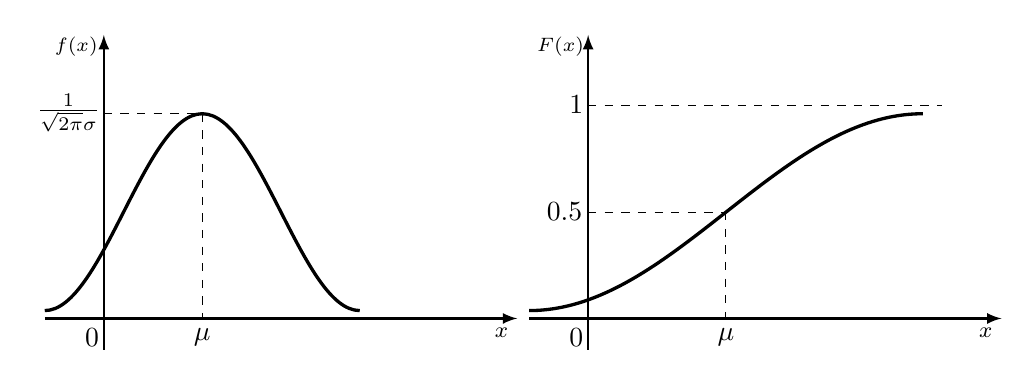
\begin{tikzpicture}


\begin{scope}[scale=0.5]

\draw [-,very thick] (-2,-1) cos(0,1.5) sin (2,4) cos(4,1.5) sin(6,-1) ;
\draw [-latex,thick] (-2.0,-1.2) -- (10,-1.2);%横轴
\draw [-latex,thick] (-0.5,-2.0) -- (-0.5,6);%纵轴
\draw [-,dashed] (2,4) -- (2,-1.2);  %%图中纵轴虚线
\draw [-,dashed] (-0.5,4) -- (2,4);  %%图中横轴虚线
\node [anchor=north] at (-0.8,-1.2) {0};
\node [anchor=north] at (2,-1.2) {$\mu$};
\node [anchor=north] at (-1.4,4.75) {$\frac{1}{\sqrt{2\pi}\sigma}$};
\node [anchor=north] at (-1.2,6.2) {\scriptsize{$f(x)$}};
\node [anchor=north] at (9.6,-1.2) {\footnotesize{$x$}};


\end{scope}

\begin{scope}[scale=0.5,xshift=35.0em]

\draw [-,very thick] (-2,-1) cos(3,1.5) sin(8,4) ;
\draw [-latex,thick] (-2.0,-1.2) -- (10,-1.2);%横轴
\draw [-latex,thick] (-0.5,-2.0) -- (-0.5,6.0);%纵轴
\draw [-,dashed] (3,1.5) -- (3,-1.2);  %%图中纵轴虚线
\draw [-,dashed] (-0.5,1.5) -- (3,1.5);  %%图中横轴虚线
\draw [-,dashed] (-0.5,4.2) -- (8.5,4.2);  %%图中横轴虚线
\node [anchor=north] at (-0.8,-1.2) {0};
\node [anchor=north] at (3,-1.2) {$\mu$};
\node [anchor=north] at (-1.1,2.0) {0.5};
\node [anchor=north] at (-0.8,4.7) {1};
\node [anchor=north] at (-1.2,6.2) {\scriptsize{$F(x)$}};
\node [anchor=north] at (9.6,-1.2) {\footnotesize{$x$}};

\end{scope}


\end{tikzpicture}
%---------------------------------------------------------------------




\caption{一个概率密度函数(左)与其对应的分布函数(右)}
\label{fig:2-1}
\end{figure}
%-------------------------------------------

\parinterval 概率密度函数反映了变量在某个区间内的概率变化快慢,概率密度函数的值是概率的变化率,该连续变量的概率分布函数也就是对概率密度函数求积分得到的结果。设$f(x) \geq 0$是连续变量$X$的概率密度函数,$X$的分布函数就可以用如下公式定义:
\begin{eqnarray}
F(x)=\int_{-\infty}^x f(x)\textrm{d}x
\label{eq:2-1}
\end{eqnarray}

%----------------------------------------------------------------------------------------
%    NEW SUB-SECTION
%----------------------------------------------------------------------------------------

\subsection{联合概率、条件概率和边缘概率}
\parinterval {\small\sffamily\bfseries{联合概率}}\index{联合概率}(Joint Probability)\index{Joint Probability}是指多个事件共同发生,每个随机变量满足各自条件的概率。如事件$A$和事件$B$的联合概率可以表示为$\funp{P}(AB)$或$\funp{P}(A\cap{B})$。{\small\sffamily\bfseries{条件概率}}\index{条件概率}(Conditional Probability)\index{Conditional Probability}是指$A$、$B$为任意的两个事件,在事件$A$已出现的前提下,事件$B$出现的概率,使用$\funp{P}(B \mid A)$表示。

\parinterval 贝叶斯法则(见\ref{sec:2.2.3}小节)是条件概率计算时的重要依据,条件概率可以表示为:
\begin{eqnarray}
\funp{P}{(B|A)} & = & \frac{\funp{P}(A\cap{B})}{\funp{P}(A)}  \nonumber \\
                           & = & \frac{\funp{P}(A)\funp{P}(B|A)}{\funp{P}(A)}  \nonumber \\
                           & = & \frac{\funp{P}(B)\funp{P}(A|B)}{\funp{P}(A)}
\label{eq:2-2}
\end{eqnarray}

\parinterval {\small\sffamily\bfseries{边缘概率}}\index{边缘概率}(Marginal Probability)\index{Marginal Probability}是和联合概率对应的,它指的是$\funp{P}(X=a)$或$\funp{P}(Y=b)$,即仅与单个随机变量有关的概率。对于离散随机变量$X$和$Y$,如果知道$\funp{P}(X,Y)$,则边缘概率$\funp{P}(X)$可以通过求和的方式得到。对于$\forall x \in X $,有:
\begin{eqnarray}
\funp{P}(X=x)=\sum_{y}  \funp{P}(X=x,Y=y)
\label{eq:2-3}
\end{eqnarray}

\parinterval 对于连续变量,边缘概率$\funp{P}(X)$需要通过积分得到,如下式所示:
\begin{eqnarray}
\funp{P}(X=x)=\int \funp{P}(x,y)\textrm{d}y
\label{eq:2-4}
\end{eqnarray}

\parinterval 为了更好地区分条件概率、边缘概率和联合概率,这里用一个图形面积的计算来举例说明。如图\ref{fig:2-2}所示,矩形$A$代表事件$X$发生所对应的所有可能状态,矩形$B$代表事件$Y$发生所对应的所有可能状态,矩形$C$代表$A$和$B$的交集,则:

\begin{itemize}
\vspace{0.5em}
\item {\small\bfnew{边缘概率}}:矩形$A$或者矩形$B$的面积。
\vspace{0.5em}
\item {\small\bfnew{联合概率}}:矩形$C$的面积。
\vspace{0.5em}
\item {\small\bfnew{条件概率}}:联合概率/对应的边缘概率,如:$\funp{P}(A \mid B)$=矩形$C$的面积/矩形B的面积。
\vspace{0.5em}
\end{itemize}

%----------------------------------------------
\begin{figure}[htp]
\centering

%%% outline
%-------------------------------------------------------------------------
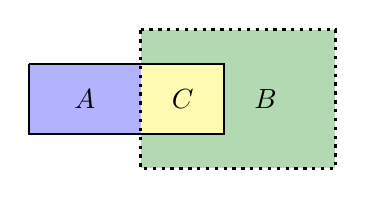
\begin{tikzpicture}



\begin{scope}[scale=1.0]
{

\node [anchor=north west,minimum width=7em, minimum height=2.5em,fill=blue!30](num1)  at (0,0) {$A$\quad \quad \quad \quad  };
\node [anchor=west,minimum width=7em, minimum height=5em,fill=ugreen!30](num2)  at ([xshift=-3em]num1.east) {\quad \quad $B$};
\node [anchor=west,minimum width=3em, minimum height=2.5em,fill=yellow!30](part1)  at (num2.west) {$C$};

\draw [-,thick] (num1.north west) -- (num1.north east) -- (num1.south east) -- (num1.south west) -- (num1.north west);
\draw [-,very thick,dotted] (num2.north west) -- (num2.north east) -- (num2.south east) -- (num2.south west) -- (num2.north west);

}
\end{scope}
\end{tikzpicture}
%---------------------------------------------------------------------


\caption{$A$、$B$、$C$事件所对应概率的图形化表示}
\label{fig:2-2}
\end{figure}
%-------------------------------------------

%----------------------------------------------------------------------------------------
%    NEW SUB-SECTION
%----------------------------------------------------------------------------------------

\subsection{链式法则} \label{sec:chain-rule}

\parinterval 条件概率公式$\funp{P}(A \mid B)=\funp{P}(AB)/\funp{P}(B)$反映了事件$B$发生的条件下事件$A$发生的概率。如果将其推广到三个事件$A$、$B$、$C$,为了计算$\funp{P}(A,B,C)$,可以运用两次$\funp{P}(A \mid B)=\funp{P}(AB)/\funp{P}(B)$,计算过程如下:
\begin{eqnarray}
\funp{P}(A,B,C) & = & \funp{P}(A \mid B ,C)\funp{P}(B,C) \nonumber \\
                           & = & \funp{P}(A \mid B,C)\funp{P}(B \mid C)\funp{P}(C)
\label{eq:2-5}
\end{eqnarray}

\parinterval 推广到$n$个事件,可以得到{\small\bfnew{链式法则}}\index{链式法则}(Chain Rule\index{Chain Rule})的公式:
\begin{eqnarray}
\funp{P}(x_1,x_2, \ldots ,x_n)=\prod_{i=1}^n \funp{P}(x_i \mid x_1, \ldots ,x_{i-1})
\label{eq:2-6}
\end{eqnarray}

\parinterval 链式法则经常被用于对事件序列的建模。比如,在事件$A$与事件$C$相互独立时,事件$A$、$B$、$C$的联合概率可以被表示为:
\begin{eqnarray}
\funp{P}(A,B,C) & = & \funp{P}(A)\funp{P}(B \mid A)\funp{P}(C \mid A,B) \nonumber \\
                & = & \funp{P}(A)\funp{P}(B \mid A)\funp{P}(C \mid B)
\label{eq:chain-rule-example}
\end{eqnarray}

%----------------------------------------------------------------------------------------
%    NEW SUB-SECTION
%----------------------------------------------------------------------------------------

\subsection{贝叶斯法则}\label{sec:2.2.3}

\parinterval 首先介绍一下全概率公式:{\small\bfnew{全概率公式}}\index{全概率公式}(Law of Total Probability)\index{Law of Total Probability}是概率论中重要的公式,它可以将一个复杂事件发生的概率分解成不同情况的小事件发生概率的和。这里先介绍一个概念——划分。集合$\Sigma$的一个划分事件为$\{B_1, \ldots ,B_n\}$是指它们满足$\bigcup_{i=1}^n B_i=S \textrm{且}B_iB_j=\varnothing , i,j=1, \ldots ,n,i\neq j$。此时事件$A$的全概率公式可以被描述为:
\begin{eqnarray}
\funp{P}(A)=\sum_{k=1}^n \funp{P}(A \mid B_k)\funp{P}(B_k)
\label{eq:2-9}
\end{eqnarray}

\parinterval 举个例子,小张从家到公司有三条路分别为$a$,$b$,$c$,选择每条路的概率分别为0.5,0.3,0.2。令:

\begin{itemize}
\vspace{0.5em}
\item $S_a$:小张选择$a$路去上班
\vspace{0.5em}
\item $S_b$:小张选择$b$路去上班
\vspace{0.5em}
\item $S_c$:小张选择$c$路去上班
\vspace{0.5em}
\item $S$:小张去上班
\vspace{0.5em}
\end{itemize}

\parinterval 显然,$S_a$,$S_b$,$S_c$是$S$的划分。如果三条路不拥堵的概率分别为$\funp{P}({S_{a}^{'}})$=0.2, $\funp{P}({S_{b}^{'}})$=0.4,$\funp{P}({S_{c}^{'}})$=0.7,那么事件$L$:小张上班没有遇到拥堵情况的概率就是:
\begin{eqnarray}
{\funp{P}(L)} &=& {\funp{P}( L| S_a )\funp{P}(S_a )+\funp{P}( L| S_b )\funp{P}(S_b )+\funp{P}( L| S_c )\funp{P}(S_c )}\nonumber \\
& = &{\funp{P}({S_{a}^{'}})\funp{P}(S_a)+\funp{P}({S_{b}^{'}})\funp{P}(S_b)+\funp{P}({S_{c}^{'}})\funp{P}(S_c) }\nonumber \\
& = &{0.36}
\label{eq:2-10}
\end{eqnarray}

\parinterval {\small\sffamily\bfseries{贝叶斯法则}}\index{贝叶斯法则}(Bayes' Rule)\index{Bayes' Rule}是概率论中的一个经典公式,通常用于已知$\funp{P}(A \mid B)$求$\funp{P}(B \mid A)$。可以表述为:设$\{B_1, \ldots ,B_n\}$是某个集合$\Sigma$的一个划分,$A$为事件,则对于$i=1, \ldots ,n$,有如下公式:
\begin{eqnarray}
\funp{P}(B_i \mid A) & = & \frac {\funp{P}(A  B_i)} { \funp{P}(A) } \nonumber \\
                                   & = & \frac {\funp{P}(A \mid B_i)\funp{P}(B_i) } { \sum_{k=1}^n\funp{P}(A \mid B_k)\funp{P}(B_k) }
\label{eq:2-11}
\end{eqnarray}

\noindent 其中,等式右端的分母部分使用了全概率公式。进一步,令$\bar{B}$表示事件$B$不发生的情况,由上式,也可以得到贝叶斯公式的另外一种写法:
\begin{eqnarray}
\funp{P}(B \mid A) & = & \frac { \funp{P}(A \mid B)\funp{P}(B) }  {\funp{P}(A)} \nonumber \\
                     & = & \frac { \funp{P}(A \mid B)\funp{P}(B) }  {\funp{P}(A \mid B)\funp{P}(B)+\funp{P}(A \mid \bar{B}) \funp{P}(\bar{B})}
\label{eq:2-12}
\end{eqnarray}

\parinterval 贝叶斯公式常用于根据已知的结果来推断使之发生的各因素的可能性。

%----------------------------------------------------------------------------------------
%    NEW SUB-SECTION
%----------------------------------------------------------------------------------------

\subsection{KL距离和熵}

%----------------------------------------------------------------------------------------
%    NEW SUBSUB-SECTION
%----------------------------------------------------------------------------------------

\subsubsection{1. 信息熵}

\parinterval 熵是热力学中的一个概念,同时也是对系统无序性的一种度量标准。在自然语言处理领域也会使用到信息熵这一概念,比如描述文字的信息量大小。一条信息的信息量可以被看作是这条信息的不确定性。如果需要确认一件非常不确定甚至于一无所知的事情,那么需要理解大量的相关信息才能进行确认;同样的,如果对某件事已经非常确定,那么就不需要太多的信息就可以把它搞清楚。如下就是两个例子,

\begin{example}
确定性和不确定性的事件

\qquad\qquad\quad“太阳从东方升起”

\qquad\qquad\quad“明天天气多云”
\label{eg:2-1}
\end{example}

\parinterval 在这两句话中,“太阳从东方升起”是一件确定性事件(在地球上),几乎不需要查阅更多信息就可以确认,因此这件事的信息熵相对较低;而“明天天气多云”这件事,需要关注天气预报,才能大概率确定这件事,它的不确定性很高,因而它的信息熵也就相对较高。因此,信息熵也是对事件不确定性的度量。进一步,一个事件$X$的{\small\bfnew{自信息}}\index{自信息}(Self-information)\index{Self-information}的表达式为:
\begin{eqnarray}
\funp{I}(x)=-\log \funp{P}(x)
\label{eq:2-13}
\end{eqnarray}

\noindent 其中,$x$是$X$的一个取值,$\funp{P}(x)$表示$x$发生的概率。自信息用来衡量单一事件发生时所包含的信息多少,当底数为e时,单位为nats,其中1nats是通过观察概率为$1/\textrm{e}$的事件而获得的信息量;当底数为2时,单位为bits或shannons。$\funp{I}(x)$和$\funp{P}(x)$的函数关系如图\ref{fig:2-3} 所示。

%----------------------------------------------
\begin{figure}[htp]
\centering
\definecolor{ublue}{rgb}{0.152,0.250,0.545}
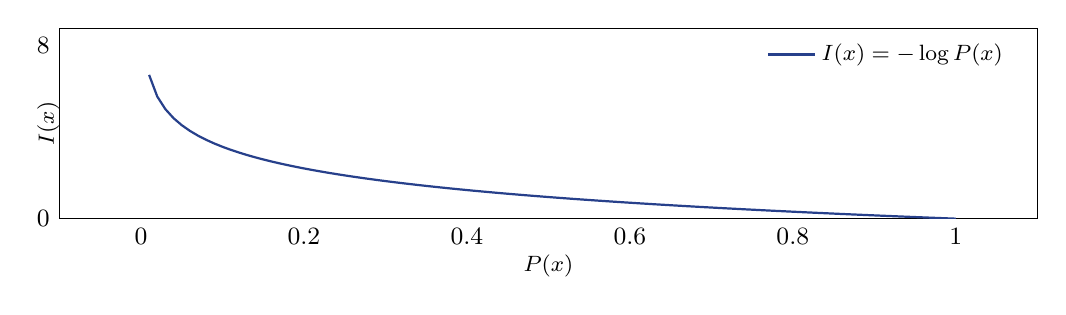
\begin{tikzpicture}
\begin{axis}[
  width=14cm,
  height=4cm,
  xlabel={{$\funp{P}(x)$}},
  ylabel={{$\funp{I}(x)$}},
  ylabel style={yshift=-1.5em,font=\footnotesize},
  xlabel style={yshift=0.3em,font=\footnotesize},
  xtick={0,0.2,...,1.0},
  ytick={0,8},
  y tick style={opacity=0},
  x tick style={opacity=0},
  domain=0.01:1,
  enlarge x limits=true,
  enlarge y limits={upper},
  legend style={draw=none,thick},
  xmin=0,
  xmax=1,
  ymin=0,
  ymax=8,
xticklabel style={font=\small}, %坐标轴字体大小
yticklabel style={font=\small}
]
\addplot[draw=ublue,samples=100,thick] {-log2(x)};
\legend{\footnotesize{$\funp{I}(x) = -\log \funp{P}(x)$}}
\end{axis}
\end{tikzpicture}

%---------------------------------------------------------------------
\caption{自信息函数$\funp{I}(x)$关于$\funp{P}(x)$的曲线}
\label{fig:2-3}
\end{figure}
%-------------------------------------------

\parinterval 自信息处理的是变量单一取值的情况。若量化整个概率分布中的不确定性或信息量,可以用信息熵,记为$\funp{H}(x)$。其公式如下:
\begin{eqnarray}
\funp{H}(x) & = & \sum_{x \in X}[ \funp{P}(x) \funp{I}(x)] \nonumber \\
              & = & - \sum_{x \in X } [\funp{P}(x)\log(\funp{P}(x)) ]
\label{eq:2-14}
\end{eqnarray}

\parinterval 一个分布的信息熵也就是从该分布中得到的一个事件的期望信息量。比如,$a$、$b$、$c$、$d$四支球队,四支队伍夺冠的概率分别是$\funp{P}_1$、$\funp{P}_2$、$\funp{P}_3$、$\funp{P}_4$,假设四只队伍的实力未知或者实力相当,那么人们就很难对比赛结果做出预测。但是,如果这四只球队中某一支球队的实力可以碾压其他球队,那么人们对比赛结果的预测就会很明确。所以对于前面这种情况,预测球队夺冠的问题的信息量较高,信息熵也相对较高;对于后面这种情况,因为结果是容易猜到的,信息量和信息熵也就相对较低。因此可以得知:分布越尖锐熵越低,分布越均匀熵越高。

%----------------------------------------------------------------------------------------
%    NEW SUBSUB-SECTION
%----------------------------------------------------------------------------------------

\subsubsection{2. KL距离}

\parinterval 如果同一个随机变量$X$上有两个概率分布$\funp{P}(x)$和$\funp{Q}(x)$,那么可以使用{\small\bfnew{Kullback-Leibler距离}}\index{Kullback-Leibler距离}或{\small\bfnew{KL距离}}\index{KL距离}(KL Distance\index{KL Distance})来衡量这两个分布的不同(也称作KL 散度)。这种度量就是{\small\bfnew{相对熵}}\index{相对熵}(Relative Entropy)\index{Relative Entropy},其公式如下:
\begin{eqnarray}
\funp{D}_{\textrm{KL}}(\funp{P}\parallel \funp{Q}) & = & \sum_{x \in X} [ \funp{P}(x)\log \frac{\funp{P}(x) }{ \funp{Q}(x) } ]  \nonumber \\
                                                                                       & = & \sum_{x \in X }[ \funp{P}(x)(\log \funp{P}(x)-\log \funp{Q}(x))]
\label{eq:2-15}
\end{eqnarray}

\parinterval 其中,概率分布$\funp{P}(x)$对应的每个事件的可能性。相对熵的意义在于:在一个事件空间里,若用概率分布$\funp{Q}(x)$来编码$\funp{P}(x)$,相比于用概率分布$\funp{P}(x)$来编码$\funp{P}(x)$时信息量增加了多少。它衡量的是同一个事件空间里两个概率分布的差异。KL距离有两条重要的性质:

\begin{itemize}
\vspace{0.5em}
\item {\small\bfnew{非负性}},即$\funp{D}_{\textrm{KL}} (\funp{P} \parallel \funp{Q}) \ge 0$,等号成立条件是$\funp{P}$和$\funp{Q}$相等。
\vspace{0.5em}
\item {\small\bfnew{不对称性}},即$\funp{D}_{\textrm{KL}} (\funp{P} \parallel \funp{Q}) \neq \funp{D}_{\textrm{KL}} (\funp{Q}  \parallel \funp{P})$,所以$\textrm{KL}$距离并不是常用的欧式空间中的距离。为了消除这种不确定性,有时也会使用$\funp{D}_{\textrm{KL}} (\funp{P}  \parallel \funp{Q})+\funp{D}_{\textrm{KL}} (\funp{Q}  \parallel \funp{P})$作为度量两个分布差异性的函数。
\vspace{0.5em}
\end{itemize}

%----------------------------------------------------------------------------------------
%    NEW SUBSUB-SECTION
%----------------------------------------------------------------------------------------

\subsubsection{3. 交叉熵}

\parinterval {\small\bfnew{交叉熵}}\index{交叉熵}(Cross-entropy)\index{Cross-entropy}是一个与KL距离密切相关的概念,它的公式是:
\begin{eqnarray}
\funp{H}(\funp{P},\funp{Q})=-\sum_{x \in X} [\funp{P}(x) \log \funp{Q}(x) ]
\label{eq:2-16}
\end{eqnarray}

\parinterval 结合相对熵公式可知,交叉熵是KL距离公式中的右半部分。因此,当概率分布$\funp{P}(x)$固定时,求关于$\funp{Q}$的交叉熵的最小值等价于求KL距离的最小值。从实践的角度来说,交叉熵与KL距离的目的相同:都是用来描述两个分布的差异。由于交叉熵计算上更加直观方便,因此在机器翻译中被广泛应用。

%----------------------------------------------------------------------------------------
%    NEW SECTION
%----------------------------------------------------------------------------------------

\sectionnewpage
\section{掷骰子游戏}

\parinterval 在阐述统计建模方法前,先看一个有趣的实例(图\ref{fig:2-4})。掷骰子,一个生活中比较常见的游戏,掷一个骰子,玩家猜一个数字,猜中就算赢。按照常识来说,随便选一个数字,获胜的概率是一样的,即所有选择的获胜概率都是$1/6$。因此这个游戏玩家很难获胜,除非运气很好。假设进行一次游戏,玩家随意选了一个数字,比如是1。当投掷30次骰子(如图\ref{fig:2-4}),发现运气不错,命中7次,好于预期($7/30 > 1/6$)。
\vspace{-0.5em}

%----------------------------------------------
\begin{figure}[htp]
\centering

\definecolor{ublue}{rgb}{0.152,0.250,0.545}
\definecolor{ugreen}{rgb}{0,0.5,0}



%%% outline
%-------------------------------------------------------------------------


    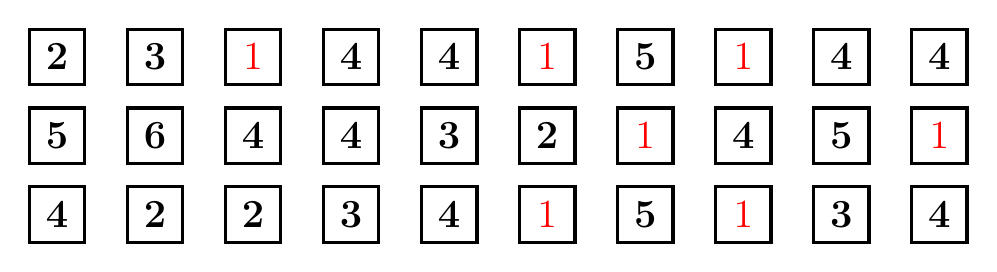
\begin{tikzpicture}

    {
    \begin{scope}
    \node[anchor=west,draw,very thick,minimum size=20pt] (s1) at (0,0) {\Large{\textbf{2}}};
    \node[anchor=west,draw,very thick,minimum size=20pt] (s2) at ([xshift=0.5cm]s1.east) {\Large{\textbf{3}}};
    \node[anchor=west,draw,very thick,minimum size=20pt] (s3) at ([xshift=0.5cm]s2.east) {\Large{{\color{red}{1}}}};
    \node[anchor=west,draw,very thick,minimum size=20pt] (s4) at ([xshift=0.5cm]s3.east) {\Large{\textbf{4}}};
    \node[anchor=west,draw,very thick,minimum size=20pt] (s5) at ([xshift=0.5cm]s4.east) {\Large{\textbf{4}}};
    \node[anchor=west,draw,very thick,minimum size=20pt] (s6) at ([xshift=0.5cm]s5.east) {\Large{{\color{red}{1}}}};
    \node[anchor=west,draw,very thick,minimum size=20pt] (s7) at ([xshift=0.5cm]s6.east) {\Large{\textbf{5}}};
    \node[anchor=west,draw,very thick,minimum size=20pt] (s8) at ([xshift=0.5cm]s7.east) {\Large{{\color{red}{1}}}};
    \node[anchor=west,draw,very thick,minimum size=20pt] (s9) at ([xshift=0.5cm]s8.east) {\Large{\textbf{4}}};
    \node[anchor=west,draw,very thick,minimum size=20pt] (s10) at ([xshift=0.5cm]s9.east) {\Large{\textbf{4}}};
    \end{scope}

    \begin{scope}[yshift=-1cm]
    \node[anchor=west,draw,very thick,minimum size=20pt] (s1) at (0,0) {\Large{\textbf{5}}};
    \node[anchor=west,draw,very thick,minimum size=20pt] (s2) at ([xshift=0.5cm]s1.east) {\Large{\textbf{6}}};
    \node[anchor=west,draw,very thick,minimum size=20pt] (s3) at ([xshift=0.5cm]s2.east) {\Large{\textbf{4}}};
    \node[anchor=west,draw,very thick,minimum size=20pt] (s4) at ([xshift=0.5cm]s3.east) {\Large{\textbf{4}}};
    \node[anchor=west,draw,very thick,minimum size=20pt] (s5) at ([xshift=0.5cm]s4.east) {\Large{\textbf{3}}};
    \node[anchor=west,draw,very thick,minimum size=20pt] (s6) at ([xshift=0.5cm]s5.east) {\Large{\textbf{2}}};
    \node[anchor=west,draw,very thick,minimum size=20pt] (s7) at ([xshift=0.5cm]s6.east) {\Large{{\color{red}{1}}}};
    \node[anchor=west,draw,very thick,minimum size=20pt] (s8) at ([xshift=0.5cm]s7.east) {\Large{\textbf{4}}};
    \node[anchor=west,draw,very thick,minimum size=20pt] (s9) at ([xshift=0.5cm]s8.east) {\Large{\textbf{5}}};
    \node[anchor=west,draw,very thick,minimum size=20pt] (s10) at ([xshift=0.5cm]s9.east) {\Large{{\color{red}{1}}}};
    \end{scope}

    \begin{scope}[yshift=-2cm]
    \node[anchor=west,draw,very thick,minimum size=20pt] (s1) at (0,0) {\Large{\textbf{4}}};
    \node[anchor=west,draw,very thick,minimum size=20pt] (s2) at ([xshift=0.5cm]s1.east) {\Large{\textbf{2}}};
    \node[anchor=west,draw,very thick,minimum size=20pt] (s3) at ([xshift=0.5cm]s2.east) {\Large{\textbf{2}}};
    \node[anchor=west,draw,very thick,minimum size=20pt] (s4) at ([xshift=0.5cm]s3.east) {\Large{\textbf{3}}};
    \node[anchor=west,draw,very thick,minimum size=20pt] (s5) at ([xshift=0.5cm]s4.east) {\Large{\textbf{4}}};
    \node[anchor=west,draw,very thick,minimum size=20pt] (s6) at ([xshift=0.5cm]s5.east) {\Large{{\color{red}{1}}}};
    \node[anchor=west,draw,very thick,minimum size=20pt] (s7) at ([xshift=0.5cm]s6.east) {\Large{\textbf{5}}};
    \node[anchor=west,draw,very thick,minimum size=20pt] (s8) at ([xshift=0.5cm]s7.east) {\Large{{\color{red}{1}}}};
    \node[anchor=west,draw,very thick,minimum size=20pt] (s9) at ([xshift=0.5cm]s8.east) {\Large{\textbf{3}}};
    \node[anchor=west,draw,very thick,minimum size=20pt] (s10) at ([xshift=0.5cm]s9.east) {\Large{\textbf{4}}};
    \end{scope}
    }
    \end{tikzpicture}



%\setlength{\belowcaptionskip}{-0.5cm}
\caption{骰子结果}
\label{fig:2-4}
\end{figure}
%-------------------------------------------

\parinterval 此时玩家的胜利似乎只能来源于运气。不过,这里的假设“随便选一个数字,获胜的概率是一样的”本身就是一个概率模型,它对骰子六个面的出现做了均匀分布假设:
\begin{eqnarray}
\funp{P}(\text{1})=\funp{P}(\text{2})= \ldots =\funp{P}(\text{5})=\funp{P}(\text{6})=1/6
\label{eq:2-17}
\end{eqnarray}

\vspace{-0.5em}
\parinterval 但是在这个游戏中没有人规定骰子是均匀的。如果骰子的六个面不均匀呢?这里可以用一种更加“聪明”的方式定义一种新的模型,即定义骰子的每一个面都以一定的概率出现,而不是相同的概率。描述如下:
\begin{eqnarray}
\funp{P}(\text{1}) &=&\theta_1 \nonumber \\
\funp{P}(\text{2}) &=&\theta_2 \nonumber \\
\funp{P}(\text{3}) &=&\theta_3 \nonumber \\
\funp{P}(\text{4}) &=&\theta_4 \nonumber \\
\funp{P}(\text{5}) &=&\theta_5 \nonumber \\
\funp{P}(\text{6}) &=&1-\sum_{1 \leq i \leq 5}\theta_i \qquad \lhd \textrm {归一性}
\label{eq:2-18}
\end{eqnarray}

\noindent 这里,$\theta_1 \sim \theta_5$可以被看作是模型的参数,因此这个模型的自由度是5。对于这样的模型,参数确定了,模型也就确定了。但是一个新的问题出现了,在定义骰子每个面的概率后,如何求出具体的概率值呢?一种常用的方法是,从大量实例中学习模型参数,这个方法也是常说的{\small\bfnew{参数估计}}\index{参数估计}(Parameter Estimation)\index{Parameter Estimation}。可以将这个不均匀的骰子先实验性地掷很多次,这可以被看作是独立同分布的若干次采样。比如投掷骰子$X$次,发现1出现$X_1$ 次,2出现$X_2$ 次,以此类推,可以得到各个面出现的次数。假设掷骰子中每个面出现的概率符合多项式分布,那么通过简单的概率论知识可以知道每个面出现概率的极大似然估计为:
\begin{eqnarray}
\funp{P}(i)=\frac {X_i}{X}
\label{eq:2-19}
\end{eqnarray}

\parinterval 当$X$足够大时,$X_i/X$可以无限逼近$\funp{P}(i)$的真实值,因此可以通过大量的实验推算出掷骰子各个面的概率的准确估计值。

\parinterval 回归到原始的问题,如果在正式开始游戏前,预先掷骰子30次,得到如图\ref{fig:2-5}的结果。

%----------------------------------------------
\begin{figure}[htp]
\centering

\definecolor{ublue}{rgb}{0.152,0.250,0.545}
\definecolor{ugreen}{rgb}{0,0.5,0}


%%% outline
%-------------------------------------------------------------------------

    \vspace{0.3em}

    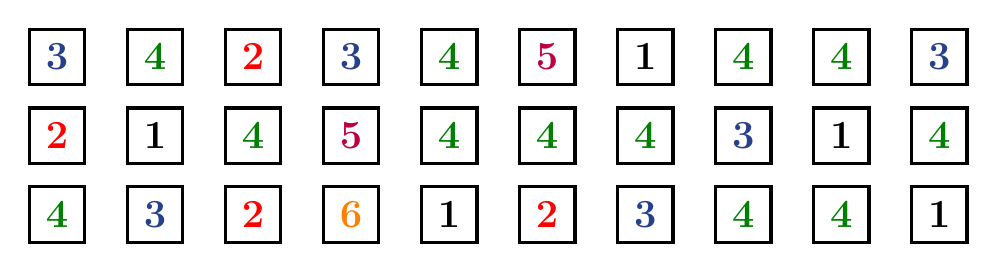
\begin{tikzpicture}

    \begin{scope}
    \node[anchor=west,draw,very thick,minimum size=20pt] (s1) at (0,0) {\Large{\textbf{{\color{ublue} 3}}}};
    \node[anchor=west,draw,very thick,minimum size=20pt] (s2) at ([xshift=0.5cm]s1.east) {\Large{\textbf{{\color{ugreen} 4}}}};
    \node[anchor=west,draw,very thick,minimum size=20pt] (s3) at ([xshift=0.5cm]s2.east) {\Large{\textbf{{\color{red} 2}}}};
    \node[anchor=west,draw,very thick,minimum size=20pt] (s4) at ([xshift=0.5cm]s3.east) {\Large{\textbf{{\color{ublue} 3}}}};
    \node[anchor=west,draw,very thick,minimum size=20pt] (s5) at ([xshift=0.5cm]s4.east) {\Large{\textbf{{\color{ugreen} 4}}}};
    \node[anchor=west,draw,very thick,minimum size=20pt] (s6) at ([xshift=0.5cm]s5.east) {\Large{\textbf{{\color{purple} 5}}}};
    \node[anchor=west,draw,very thick,minimum size=20pt] (s7) at ([xshift=0.5cm]s6.east) {\Large{\textbf{1}}};
    \node[anchor=west,draw,very thick,minimum size=20pt] (s8) at ([xshift=0.5cm]s7.east) {\Large{\textbf{{\color{ugreen} 4}}}};
    \node[anchor=west,draw,very thick,minimum size=20pt] (s9) at ([xshift=0.5cm]s8.east) {\Large{\textbf{{\color{ugreen} 4}}}};
    \node[anchor=west,draw,very thick,minimum size=20pt] (s10) at ([xshift=0.5cm]s9.east) {\Large{\textbf{{\color{ublue} 3}}}};
    \end{scope}

    \begin{scope}[yshift=-1cm]
    \node[anchor=west,draw,very thick,minimum size=20pt] (s1) at (0,0) {\Large{\textbf{{\color{red} 2}}}};
    \node[anchor=west,draw,very thick,minimum size=20pt] (s2) at ([xshift=0.5cm]s1.east) {\Large{\textbf{1}}};
    \node[anchor=west,draw,very thick,minimum size=20pt] (s3) at ([xshift=0.5cm]s2.east) {\Large{\textbf{{\color{ugreen} 4}}}};
    \node[anchor=west,draw,very thick,minimum size=20pt] (s4) at ([xshift=0.5cm]s3.east) {\Large{\textbf{{\color{purple} 5}}}};
    \node[anchor=west,draw,very thick,minimum size=20pt] (s5) at ([xshift=0.5cm]s4.east) {\Large{\textbf{{\color{ugreen} 4}}}};
    \node[anchor=west,draw,very thick,minimum size=20pt] (s6) at ([xshift=0.5cm]s5.east) {\Large{\textbf{{\color{ugreen} 4}}}};
    \node[anchor=west,draw,very thick,minimum size=20pt] (s7) at ([xshift=0.5cm]s6.east) {\Large{\textbf{{\color{ugreen} 4}}}};
    \node[anchor=west,draw,very thick,minimum size=20pt] (s8) at ([xshift=0.5cm]s7.east) {\Large{\textbf{{\color{ublue} 3}}}};
    \node[anchor=west,draw,very thick,minimum size=20pt] (s9) at ([xshift=0.5cm]s8.east) {\Large{\textbf{1}}};
    \node[anchor=west,draw,very thick,minimum size=20pt] (s10) at ([xshift=0.5cm]s9.east) {\Large{\textbf{{\color{ugreen} 4}}}};
    \end{scope}

    \begin{scope}[yshift=-2cm]
    \node[anchor=west,draw,very thick,minimum size=20pt] (s1) at (0,0) {\Large{\textbf{{\color{ugreen} 4}}}};
    \node[anchor=west,draw,very thick,minimum size=20pt] (s2) at ([xshift=0.5cm]s1.east) {\Large{\textbf{{\color{ublue} 3}}}};
    \node[anchor=west,draw,very thick,minimum size=20pt] (s3) at ([xshift=0.5cm]s2.east) {\Large{\textbf{{\color{red} 2}}}};
    \node[anchor=west,draw,very thick,minimum size=20pt] (s4) at ([xshift=0.5cm]s3.east) {\Large{\textbf{{\color{orange} 6}}}};
    \node[anchor=west,draw,very thick,minimum size=20pt] (s5) at ([xshift=0.5cm]s4.east) {\Large{\textbf{1}}};
    \node[anchor=west,draw,very thick,minimum size=20pt] (s6) at ([xshift=0.5cm]s5.east) {\Large{\textbf{{\color{red} 2}}}};
    \node[anchor=west,draw,very thick,minimum size=20pt] (s7) at ([xshift=0.5cm]s6.east) {\Large{\textbf{{\color{ublue} 3}}}};
    \node[anchor=west,draw,very thick,minimum size=20pt] (s8) at ([xshift=0.5cm]s7.east) {\Large{\textbf{{\color{ugreen} 4}}}};
    \node[anchor=west,draw,very thick,minimum size=20pt] (s9) at ([xshift=0.5cm]s8.east) {\Large{\textbf{{\color{ugreen} 4}}}};
    \node[anchor=west,draw,very thick,minimum size=20pt] (s10) at ([xshift=0.5cm]s9.east) {\Large{\textbf{1}}};
    \end{scope}

    \end{tikzpicture}

%---------------------------------------------------------------------



\caption{实验性投掷骰子的结果}
\label{fig:2-5}
\end{figure}
%-------------------------------------------

\parinterval 此时,可以注意到,这是一个有倾向性的模型(图 \ref{fig:2-6}):在这样的预先实验基础上,可以知道这个骰子是不均匀的,如果用这个骰子玩掷骰子游戏,选择数字4获胜的可能性是最大的。

%----------------------------------------------
\begin{figure}[htp]
\centering

\definecolor{ublue}{rgb}{0.152,0.250,0.545}
\definecolor{ugreen}{rgb}{0,0.5,0}


%%% outline
%-------------------------------------------------------------------------

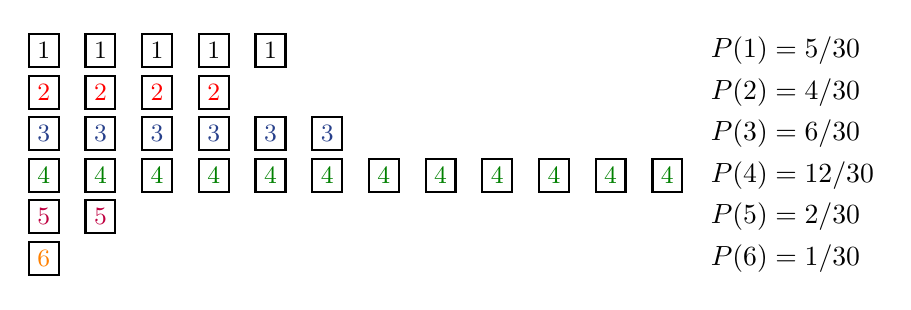
\begin{tikzpicture}[scale=0.6]
\begin{scope}
{\small
\foreach \i in {1,...,5}{
    \node [draw,thick,minimum size=10pt] at (1.2*\i,0) {1};
}
}
\node [anchor=west] at (43em,0) {$\funp{P}(\text{1}) = 5/30$};
\end{scope}

\begin{scope}[yshift=-2.5em]
{\small
\foreach \i in {1,...,4}{
    \node [draw,thick,minimum size=10pt] at (1.2*\i,0) {{\color{red} 2}};
}
}
\node [anchor=west] at (43em,0) {$\funp{P}(\text{2}) = 4/30$};
\end{scope}

\begin{scope}[yshift=-5.0em]
{\small
\foreach \i in {1,...,6}{
    \node [draw,thick,minimum size=10pt] at (1.2*\i,0) {{\color{ublue} 3}};
}
}
\node [anchor=west] at (43em,0) {$\funp{P}(\text{3}) = 6/30$};
\end{scope}

\begin{scope}[yshift=-7.5em]
{\small
\foreach \i in {1,...,12}{
    \node [draw,thick,minimum size=10pt] at (1.2*\i,0) {{\color{ugreen} 4}};
}
}
\node [anchor=west] at (43em,0) {$\funp{P}(\text{4}) = 12/30$};
\end{scope}

\begin{scope}[yshift=-10.0em]
{\small
\foreach \i in {1,...,2}{
    \node [draw,thick,minimum size=10pt] at (1.2*\i,0) {{\color{purple} 5}};
}
}
\node [anchor=west] at (43em,0) {$\funp{P}(\text{5}) = 2/30$};
\end{scope}

\begin{scope}[yshift=-12.5em]
{\small
\foreach \i in {1,...,1}{
    \node [draw,thick,minimum size=10pt] at (1.2*\i,0) {{\color{orange} 6}};
}
}
\node [anchor=west] at (43em,0) {$\funp{P}(\text{6}) = 1/30$};
\end{scope}

\end{tikzpicture}





\caption{投骰子模型}
\label{fig:2-6}
\end{figure}
%-------------------------------------------

\parinterval 与上面这个掷骰子游戏类似,世界上的事物并不是平等出现的。在“公平”的世界中,没有任何一个模型可以学到有价值的事情。从机器学习的角度来看,所谓的“不公平”实际上是客观事物中蕴含的一种{\small\sffamily\bfseries{偏置}}\index{偏置}(Bias)\index{Bias},也就是很多事情天然地就有对某些情况有倾向。而图像处理、自然语言处理等问题中绝大多数都存在着偏置。比如,当翻译一个英语单词的时候,它最可能的翻译结果往往就是那几个词。设计统计模型的目的正是要学习这种偏置,之后利用这种偏置对新的问题做出足够好的决策。

\parinterval 在处理自然语言问题时,为了评价哪些词更容易在一个句子中出现,或者哪些句子在某些语境下更合理,常常也会使用统计方法对词或句子出现的可能性建模。与掷骰子游戏类似,词出现的概率可以这样理解:每个单词的出现就好比掷一个巨大的骰子,与前面的例子中有所不同的是:

\begin{itemize}
\vspace{0.5em}
\item 骰子有很多个面,每个面代表一个单词。
\vspace{0.5em}
\item 骰子是不均匀的,代表常用单词的那些面的出现次数会远远多于罕见单词。
\vspace{0.5em}
\end{itemize}

\parinterval 如果投掷这个新的骰子,可能会得到图\ref{fig:2-7}这样的结果。如果把这些数字换成汉语中的词,比如:
\vspace{0.5em}

\parinterval 88\; = \; 这

\parinterval 87\; = \; 是

\parinterval 45\; = \; 一

\parinterval  \ldots
\vspace{0.5em}

\parinterval 就可以得到图\ref{fig:2-8}所示的结果。于是,可以假设有一个不均匀的多面骰子,每个面都对应一个单词。在获取一些文本数据后,可以统计每个单词出现的次数,进而利用极大似然估计推算出每个单词在语料库中出现的概率的估计值。图\ref{fig:2-9}给出了一个实例

%----------------------------------------------
\begin{figure}[htp]
\centering

\definecolor{ublue}{rgb}{0.152,0.250,0.545}
\definecolor{ugreen}{rgb}{0,0.5,0}



%%% outline
%-------------------------------------------------------------------------


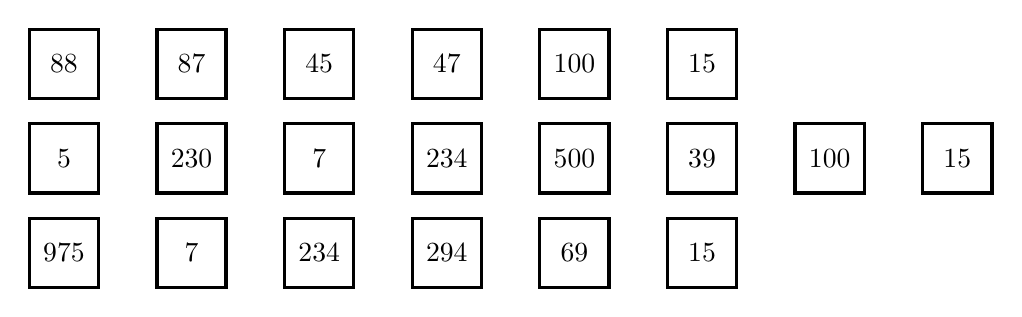
\begin{tikzpicture}

{
\begin{scope}
\node[anchor=west,draw,very thick,minimum size=25pt] (s1) at (0,0) {{88}};
\node[anchor=west,draw,very thick,minimum size=25pt] (s2) at ([xshift=0.7cm]s1.east) {{87}};
\node[anchor=west,draw,very thick,minimum size=25pt] (s3) at ([xshift=0.7cm]s2.east) {{45}};
\node[anchor=west,draw,very thick,minimum size=25pt] (s4) at ([xshift=0.7cm]s3.east) {{47}};
\node[anchor=west,draw,very thick,minimum size=25pt, inner sep=0] (s5) at ([xshift=0.7cm]s4.east) {{100}};
\node[anchor=west,draw,very thick,minimum size=25pt] (s6) at ([xshift=0.7cm]s5.east) {{15}};
\end{scope}

\begin{scope}[yshift=-1.2cm]
\node[anchor=west,draw,very thick,minimum size=25pt, inner sep=0] (s1) at (0,0) {{5}};
\node[anchor=west,draw,very thick,minimum size=25pt, inner sep=0] (s2) at ([xshift=0.7cm]s1.east) {{230}};
\node[anchor=west,draw,very thick,minimum size=25pt] (s3) at ([xshift=0.7cm]s2.east) {{7}};
\node[anchor=west,draw,very thick,minimum size=25pt, inner sep=0] (s4) at ([xshift=0.7cm]s3.east) {{234}};
\node[anchor=west,draw,very thick,minimum size=25pt, inner sep=0] (s5) at ([xshift=0.7cm]s4.east) {{500}};
\node[anchor=west,draw,very thick,minimum size=25pt] (s6) at ([xshift=0.7cm]s5.east) {{39}};
\node[anchor=west,draw,very thick,minimum size=25pt, inner sep=0] (s7) at ([xshift=0.7cm]s6.east) {{100}};
\node[anchor=west,draw,very thick,minimum size=25pt] (s8) at ([xshift=0.7cm]s7.east) {{15}};

\end{scope}

\begin{scope}[yshift=-2.4cm]
\node[anchor=west,draw,very thick,minimum size=25pt, inner sep=0] (s1) at (0,0) {{975}};
\node[anchor=west,draw,very thick,minimum size=25pt] (s2) at ([xshift=0.7cm]s1.east) {{7}};
\node[anchor=west,draw,very thick,minimum size=25pt, inner sep=0] (s3) at ([xshift=0.7cm]s2.east) {{234}};
\node[anchor=west,draw,very thick,minimum size=25pt, inner sep=0] (s4) at ([xshift=0.7cm]s3.east) {{294}};
\node[anchor=west,draw,very thick,minimum size=25pt, inner sep=0] (s5) at ([xshift=0.7cm]s4.east) {{69}};
\node[anchor=west,draw,very thick,minimum size=25pt] (s6) at ([xshift=0.7cm]s5.east) {{15}};

\end{scope}

}


\end{tikzpicture}





\caption{投掷一个很多面骰子的结果}
\label{fig:2-7}
\end{figure}
%-------------------------------------------

%----------------------------------------------
\begin{figure}[htp]
\centering

\definecolor{ublue}{rgb}{0.152,0.250,0.545}
\definecolor{ugreen}{rgb}{0,0.5,0}



%%% outline
%-------------------------------------------------------------------------
\begin{tikzpicture}
\begin{scope}
\node[anchor=west,draw,very thick,minimum size=25pt] (s1) at (0,0) {这};
\node[anchor=west,draw,very thick,minimum size=25pt] (s2) at ([xshift=0.55cm]s1.east) {是};
\node[anchor=west,draw,very thick,minimum size=25pt] (s3) at ([xshift=0.55cm]s2.east) {一};
\node[anchor=west,draw,very thick,minimum size=25pt] (s4) at ([xshift=0.55cm]s3.east) {种};
\node[anchor=west,draw,very thick,minimum size=25pt, inner sep=0] (s5) at ([xshift=0.55cm]s4.east) {\small{数据}};
\node[anchor=west,draw,very thick,minimum size=25pt] (s6) at ([xshift=0.55cm]s5.east) {。};
\node[anchor=west] (s7) at ([xshift=0.55cm]s6.east) {...};
\end{scope}

\begin{scope}[yshift=-1.2cm]
\node[anchor=west,draw,very thick,minimum size=25pt, inner sep=0] (s1) at (0,0) {现在};
\node[anchor=west,draw,very thick,minimum size=25pt, inner sep=0] (s2) at ([xshift=0.55cm]s1.east) {已经};
\node[anchor=west,draw,very thick,minimum size=25pt] (s3) at ([xshift=0.55cm]s2.east) {有};
\node[anchor=west,draw,very thick,minimum size=25pt, inner sep=0] (s4) at ([xshift=0.55cm]s3.east) {不少};
\node[anchor=west,draw,very thick,minimum size=25pt, inner sep=0] (s5) at ([xshift=0.55cm]s4.east) {\small{可}};
\node[anchor=west,draw,very thick,minimum size=25pt] (s6) at ([xshift=0.55cm]s5.east) {用};
\node[anchor=west,draw,very thick,minimum size=25pt, inner sep=0] (s7) at ([xshift=0.55cm]s6.east) {数据};
\node[anchor=west,draw,very thick,minimum size=25pt] (s8) at ([xshift=0.55cm]s7.east) {。};
\node[anchor=west] (s9) at ([xshift=0.55cm]s8.east) {...};
\end{scope}

\begin{scope}[yshift=-2.4cm]
\node[anchor=west,draw,very thick,minimum size=25pt, inner sep=0] (s1) at (0,0) {确实};
\node[anchor=west,draw,very thick,minimum size=25pt] (s2) at ([xshift=0.55cm]s1.east) {有};
\node[anchor=west,draw,very thick,minimum size=25pt, inner sep=0] (s3) at ([xshift=0.55cm]s2.east) {很};
\node[anchor=west,draw,very thick,minimum size=25pt, inner sep=0] (s4) at ([xshift=0.55cm]s3.east) {多};
\node[anchor=west,draw,very thick,minimum size=25pt, inner sep=0] (s5) at ([xshift=0.55cm]s4.east) {疑问};
\node[anchor=west,draw,very thick,minimum size=25pt] (s6) at ([xshift=0.55cm]s5.east) {。};
\node[anchor=west] (s7) at ([xshift=0.55cm]s6.east) {...};
\end{scope}

\end{tikzpicture}
	

%---------------------------------------------------------------------




\setlength{\belowcaptionskip}{-0.2cm}
\caption{掷骰子游戏中把数字换成汉字后的结果}
\label{fig:2-8}
\end{figure}
%-------------------------------------------

%----------------------------------------------
\begin{figure}[htp]
\centering


\definecolor{ublue}{rgb}{0.152,0.250,0.545}
\definecolor{ugreen}{rgb}{0,0.5,0}




%%% outline
%-------------------------------------------------------------------------
\begin{tikzpicture}

\node [anchor=west] (label1) at (0,0) {总词数:$6 + 8 + 5 = 20$};
\node [anchor=north west] (p1) at (label1.south west) {$\funp{P}(\textrm{很})=1/20=0.05$};
\node [anchor=north west] (p2) at (p1.south west) {$\funp{P}(\textrm{。})=3/20=0.15$};
\node [anchor=north west] (p3) at (p2.south west) {$\funp{P}(\textrm{确实})=1/20=0.05$};



\node [anchor=north west] (label11) at ([xshift=18.0em,yshift=1.63em]label1.south west) {更多数据-总词数:1百万个词};
\node [anchor=north west] (p12) at (label11.south west) {$\funp{P}(\textrm{很})=0.000010$};
\node [anchor=north west] (p22) at (p12.south west) {$\funp{P}(\textrm{。})=0.001812$};
\node [anchor=north west] (p32) at (p22.south west) {$\funp{P}(\textrm{确实})=0.000001$};



\begin{pgfonlayer}{background}
{
\node[rectangle,draw=ublue, inner sep=0mm] [fit =(label1)(label11)(p3)(p32)] {};
}
\end{pgfonlayer}

\end{tikzpicture}
%---------------------------------------------------------------------




\caption{单词概率的估计结果}
\label{fig:2-9}
\end{figure}
%-------------------------------------------

\parinterval 通过这个学习过程,就可以得到每个词出现的概率,成功使用统计方法对“单词的频率”这个问题进行建模。那么该如何计算一个句子的概率呢?在自然语言处理领域中,句子可以被看作是由单词组成的序列,因而句子的概率可以被建模为若干单词的联合概率,即$\funp{P}(w_1 w_2 \ldots w_m)$。其中,$w_i$表示句子中的一个单词。

\parinterval 为了求$\funp{P}(w_1 w_2 \ldots w_m)$,最直接的方式是统计所有可能出现的词串$w_1 w_2 \ldots w_m$在数据中出现的次数$c(w_1 w_2 \ldots w_m)$,之后利用极大似然估计计算$\funp{P}(w_1 w_2 \ldots w_m)$:
\begin{eqnarray}
\funp{P}(w_1 w_2 \ldots w_m) & = & \frac{c(w_1 w_2 \ldots w_m)}{\sum_{w^{'}_1, w^{'}_2,...,w^{'}_m \in V} c(w^{'}_1 w^{'}_2 \ldots w^{'}_m)} \label{eq:seq-mle}
\label{eq:2-20}
\end{eqnarray}

\noindent 其中,$V$为词汇表。本质上,这个方法和计算单词出现概率$\funp{P}(w_i)$的方法是一样的。但是这里的问题是:当$m$较大时,词串$w_1 w_2 \ldots w_m$可能非常低频,甚至在数据中没有出现过。这时,由于$c(w_1 w_2 \ldots w_m) \approx 0$,公式\eqref{eq:seq-mle}的结果会不准确,甚至产生0概率的情况。这是观测低频事件时经常出现的问题。对于这个问题,另一种思路是对多个联合出现的事件进行独立性假设,这里可以假设$w_1$、$w_2\ldots w_m$的出现是相互独立的,于是:
\begin{eqnarray}
\funp{P}(w_1 w_2 \ldots w_m) & = & \funp{P}(w_1) \funp{P}(w_2) \ldots \funp{P}(w_m) \label{eq:seq-independ}
\label{eq:2-21}
\end{eqnarray}

\noindent 这样,单词序列的出现的概率被转化为每个单词概率的乘积。由于单词的概率估计是相对准确的,因此整个序列的概率会比较合理。但是,这种独立性假设也破坏了句子中单词之间的依赖关系,造成概率估计结果的偏差。那如何更加合理的计算一个单词序列的概率呢?下面介绍的$n$-gram语言建模方法可以很好地回答这个问题。

%----------------------------------------------------------------------------------------
%    NEW SECTION
%----------------------------------------------------------------------------------------

\sectionnewpage
\section{$n$-gram语言模型}

\parinterval 在骰子游戏中,可以通过一种统计的方式,估计出在文本中词和句子出现的概率。但是在计算句子概率时往往会因为句子的样本过少而无法正确估计出句子出现的概率。为了解决这个问题,这里引入了计算整个单词序列概率$\funp{P}(w_1 w_2 \ldots w_m)$的方法\ \dash \ 统计语言模型。下面将重点介绍$n$-gram语言模型。它是一种经典的统计语言模型,而且在机器翻译及其他自然语言处理任务中有非常广泛的应用。

%----------------------------------------------------------------------------------------
%    NEW SUB-SECTION
%----------------------------------------------------------------------------------------

\subsection{建模}

\parinterval {\small\sffamily\bfseries{语言模型}}\index{语言模型}(Language Model)\index{Language Model}的目的是描述文字序列出现的规律,其对问题建模的过程被称作{\small\sffamily\bfseries{语言建模}}\index{语言建模}(Language Modeling)\index{Language Modeling}。如果使用统计建模的方式,语言模型可以被定义为计算$\funp{P}(w_1 w_2 \ldots w_m)$的问题,也就是计算整个词序列$w_1 w_2 \ldots w_m$出现的可能性大小。具体定义如下,

%----------------------------------------------
% 定义3.1
\vspace{0.5em}
\begin{definition}[]
词汇表V上的语言模型是一个函数$\funp{P}(w_1 w_2 \ldots w_m)$,它表示$V^+$上的一个概率分布。其中,对于任何词串$w_1 w_2 \ldots w_m\in{V^+}$,有$\funp{P}(w_1 w_2 \ldots w_m)\geq{0}$。而且对于所有的词串,函数满足归一化条件$\sum{_{w_1 w_2 \ldots w_m\in{V^+}}\funp{P}(w_1 w_2 \ldots w_m)}=1$。
\end{definition}
%-------------------------------------------

\parinterval 直接求$\funp{P}(w_1 w_2 \ldots w_m)$并不简单,因为如果把整个词串$w_1 w_2 \ldots w_m$作为一个变量,模型的参数量会非常大。$w_1 w_2 \ldots w_m$有$|V|^m$种可能性,这里$|V|$表示词汇表大小。显然,当$m$ 增大时,模型的复杂度会急剧增加,甚至都无法进行存储和计算。既然把$w_1 w_2 \ldots w_m$作为一个变量不好处理,就可以考虑对这个序列的生成过程进行分解。使用链式法则(见\ref{sec:chain-rule} 节),很容易得到:
\begin{eqnarray}
\funp{P}(w_1 w_2 \ldots w_m)=\funp{P}(w_1)\funp{P}(w_2|w_1)\funp{P}(w_3|w_1 w_2) \ldots \funp{P}(w_m|w_1 w_2 \ldots w_{m-1})
\label{eq:2-22}
\end{eqnarray}

\parinterval 这样,$w_1 w_2 \ldots w_m$的生成可以被看作是逐个生成每个单词的过程,即首先生成$w_1$,然后根据$w_1$再生成$w_2$,然后根据$w_1 w_2$再生成$w_3$,以此类推,直到根据所有前$m-1$个词生成序列的最后一个单词$w_m$。这个模型把联合概率$\funp{P}(w_1 w_2 \ldots w_m)$分解为多个条件概率的乘积,虽然对生成序列的过程进行了分解,但是模型的复杂度和以前是一样的,比如,$\funp{P}(w_m|w_1 w_2 \ldots w_{m-1})$ 仍然不好计算。

\parinterval 换一个角度看,$\funp{P}(w_m|w_1 w_2 \ldots w_{m-1})$体现了一种基于“历史”的单词生成模型,也就是把前面生成的所有单词作为“历史”,并参考这个“历史”生成当前单词。但是这个“历史”的长度和整个序列长度是相关的,也是一种长度变化的历史序列。为了化简问题,一种简单的想法是使用定长历史,比如,每次只考虑前面$n-1$个历史单词来生成当前单词。这就是$n$-gram语言模型,其中$n$-gram 表示$n$个连续单词构成的单元,也被称作{\small\bfnew{$n$元语法单元}}\index{$n$元语法单元}。这个模型的数学描述如下:
\begin{eqnarray}
\funp{P}(w_m|w_1 w_2 \ldots w_{m-1}) = \funp{P}(w_m|w_{m-n+1} \ldots w_{m-1})
\label{eq:2-23}
\end{eqnarray}

\parinterval 如表\ref{tab:2-2}所示,整个序列$w_1 w_2 \ldots w_m$的生成概率可以被重新定义为:

%------------------------------------------------------
\begin{table}[htp]{
\begin{center}
\caption{基于$n$-gram的序列生成概率}
{\footnotesize
\begin{tabular}{l|l|l |l|l}
链式法则 & 1-gram & 2-gram & $ \ldots $ & $n$-gram\\
 \hline
\rule{0pt}{10pt} $\funp{P}(w_1 w_2 \ldots w_m)$ = & $\funp{P}(w_1 w_2 \ldots w_m)$ = & $\funp{P}(w_1 w_2 \ldots w_m)$ = & $ \ldots $ & $\funp{P}(w_1 w_2 \ldots w_m)$ = \\
\rule{0pt}{10pt} $\funp{P}(w_1)\times$ & $\funp{P}(w_1)\times$ & $\funp{P}(w_1)\times$  & $ \ldots $ & $\funp{P}(w_1)\times$ \\
\rule{0pt}{10pt} $\funp{P}(w_2|w_1)\times$ & $\funp{P}(w_2)\times$ & $\funp{P}(w_2|w_1)\times$ & $ \ldots $ & $\funp{P}(w_2|w_1)\times$\\
\rule{0pt}{10pt} $\funp{P}(w_3|w_1 w_2)\times$ & $\funp{P}(w_3)\times$ & $\funp{P}(w_3|w_2)\times$ & $ \ldots $ & $\funp{P}(w_3|w_1 w_2)\times$ \\
\rule{0pt}{10pt} $\funp{P}(w_4|w_1 w_2 w_3)\times$ & $\funp{P}(w_4)\times$ & $\funp{P}(w_4|w_3)\times$ & $ \ldots $ & $\funp{P}(w_4|w_1 w_2 w_3)\times$ \\
\rule{0pt}{10pt} $ \ldots $ & $ \ldots $ & $ \ldots $ & $ \ldots $ & $ \ldots $ \\
\rule{0pt}{10pt} $\funp{P}(w_m|w_1  \ldots  w_{m-1})$ & $\funp{P}(w_m)$ & $\funp{P}(w_m|w_{m-1})$ & $ \ldots $ & $\funp{P}(w_m|w_{m-n+1}  \ldots  w_{m-1})$
\end{tabular}
}
\label{tab:2-2}
\end{center}
}
\end{table}
%------------------------------------------------------

\parinterval 可以看到,1-gram语言模型只是$n$-gram语言模型的一种特殊形式。基于独立性假设,1-gram假定当前单词出现与否与任何历史都无关,这种方法大大化简了求解句子概率的复杂度。比如,上一节中公式\eqref{eq:seq-independ}就是一个1-gram语言模型。但是,句子中的单词并非完全相互独立的,这种独立性假设并不能完美地描述客观世界的问题。如果需要更精确地获取句子的概率,就需要使用更长的“历史”信息,比如,2-gram、3-gram、甚至更高阶的语言模型。

\parinterval $n$-gram的优点在于,它所使用的历史信息是有限的,即$n-1$个单词。这种性质也反映了经典的马尔可夫链的思想\upcite{liuke-markov-2004,resnick1992adventures},有时也被称作马尔可夫假设或者马尔可夫属性。因此$n$-gram也可以被看作是变长序列上的一种马尔可夫模型,比如,2-gram语言模型对应着1阶马尔可夫模型,3-gram语言模型对应着2阶马尔可夫模型,以此类推。

\parinterval 那么,如何计算$\funp{P}(w_m|w_{m-n+1}  \ldots  w_{m-1})$呢?有很多种选择,比如:

\begin{itemize}
\vspace{0.5em}
\item {\small\bfnew{基于频次的方法}}\index{基于频次的方法}。直接利用词序列在训练数据中出现的频次计算出$\funp{P}(w_m|w_{m-n+1}$\\$ \ldots  w_{m-1})$:
\begin{eqnarray}
\funp{P}(w_m|w_{m-n+1} \ldots w_{m-1})=\frac{c(w_{m-n+1} \ldots w_m)}{c(w_{m-n+1} \ldots w_{m-1})}
\label{eq:2-24}
\vspace{0.5em}
\end{eqnarray}

\noindent 其中,$c(\cdot)$是在训练数据中统计频次的函数。

\vspace{0.5em}
\item {\small\bfnew{人工神经网络方法}}\index{人工神经网络方法}。构建一个人工神经网络估计$\funp{P}(w_m|w_{m-n+1}  \ldots  w_{m-1})$的值,比如,可以构建一个前馈神经网络来对$n$-gram进行建模。
\end{itemize}
\vspace{0.5em}

\parinterval 极大似然估计方法(基于频次的方法)和掷骰子游戏中介绍的统计单词概率的方法是一致的,它的核心是使用$n$-gram出现的频次进行参数估计。基于人工神经网络的方法在近些年也非常受关注,它直接利用多层神经网络对问题的输入$w_{m-n+1} \ldots w_{m-1}$和输出$\funp{P}(w_m|w_{m-n+1}  \ldots  w_{m-1})$进行建模,而模型的参数通过网络中神经元之间连接的权重进行体现。严格来说,基于人工神经网络的方法并不算基于$n$-gram的方法,或者说它并没有显性记录$n$-gram的生成概率,也不依赖$n$-gram的频次进行参数估计。为了保证内容的连贯性,接下来仍以传统$n$-gram语言模型为基础进行讨论,基于人工神经网络的方法将会在{\chapternine}进行详细介绍。

\parinterval $n$-gram语言模型的使用非常简单。可以直接用它来对词序列出现的概率进行计算。比如,可以使用一个2-gram语言模型计算一个句子出现的概率,其中单词之间用斜杠分隔,如下:
\begin{eqnarray}
 & &\funp{P}_{2\textrm{-gram}}{(\textrm{确实/现在/数据/很/多})} \nonumber \\
&= & \funp{P}(\textrm{确实}) \times \funp{P}(\textrm{现在}|\textrm{确实})\times \funp{P}(\textrm{数据}|\textrm{现在}) \times \nonumber \\
&  & \funp{P}(\textrm{很}|\textrm{数据})\times \funp{P}(\textrm{多}|\textrm{很})
\label{eq:2-25}
\end{eqnarray}

\parinterval 以$n$-gram语言模型为代表的统计语言模型的应用非常广泛。除了将要在第三章中介绍的全概率分词方法,在文本生成、信息检索、摘要等自然语言处理任务中,语言模型都有举足轻重的地位。包括近些年非常受关注的预训练模型,本质上也是统计语言模型。这些技术都会在后续章节进行介绍。值得注意的是,统计语言模型为解决自然语言处理问题提供了一个非常好的建模思路,即:把整个序列生成的问题转化为逐个生成单词的问题。实际上,这种建模方式会被广泛地用于机器翻译建模,在统计机器翻译和神经机器翻译中都会有具体的体现。

%----------------------------------------------------------------------------------------
%    NEW SUB-SECTION
%----------------------------------------------------------------------------------------

\subsection{参数估计和平滑算法}

\parinterval 对于$n$-gram语言模型,每个$\funp{P}(w_m|w_{m-n+1} \ldots w_{m-1})$都可以被看作是模型的{\small\bfnew{参数}}\index{参数}(Parameter\index{Parameter})。而$n$-gram语言模型的一个核心任务是估计这些参数的值,即参数估计。通常,参数估计可以通过在数据上的统计得到。一种简单的方法是:给定一定数量的句子,统计每个$n$-gram 出现的频次,并利用公式\eqref{eq:2-24}得到每个参数$\funp{P}(w_m|w_{m-n+1} \ldots w_{m-1})$的值。这个过程也被称作模型的{\small\bfnew{训练}}\index{训练}(Training\index{Training})。对于自然语言处理任务来说,统计模型的训练是至关重要的。在本书后面的内容中也会看到,不同的问题可能需要不同的模型以及不同的模型训练方法,并且很多研究工作也都集中在优化模型训练的效果上。

\parinterval 回到$n$-gram语言模型上。前面所使用的参数估计方法并不完美,因为它无法很好地处理低频或者未见现象。比如,在式\eqref{eq:2-25}所示的例子中,如果语料中从没有“确实”和“现在”两个词连续出现的情况,即$c(\textrm{确实}/\textrm{现在})=0$。 那么使用2-gram 计算句子“确实/现在/数据/很/多”的概率时,会出现如下情况:
\begin{eqnarray}
\funp{P}(\textrm{现在}|\textrm{确实}) & =  & \frac{c(\textrm{确实}/\textrm{现在})}{c(\textrm{确实})} \nonumber \\
                                                                     & =  & \frac{0}{c(\textrm{确实})} \nonumber \\
                                                                     & =  & 0
\label{eq:2-26}
\end{eqnarray}

\parinterval 显然,这个结果是不合理的。因为即使语料中没有 “确实”和“现在”两个词连续出现,这种搭配也是客观存在的。这时简单地用极大似然估计得到概率却是0,导致整个句子出现的概率为0。 更常见的问题是那些根本没有出现在词表中的词,称为{\small\sffamily\bfseries{未登录词}}\index{未登录词}(Out-of-vocabulary Word,OOV Word)\index{Out-of-vocabulary Word},比如一些生僻词,可能模型训练阶段从来没有看到过,这时模型仍然会给出0概率。图\ref{fig:2-10}展示了一个真实语料库中词语出现频次的分布,可以看到绝大多数词都是低频词。

%----------------------------------------------
\begin{figure}[htp]
    \centering
\definecolor{ublue}{rgb}{0.152,0.250,0.545}
\begin{tikzpicture}
\begin{axis}[
  width=13cm,
  height=5.5cm,
  xlabel={WikiText-103上的词表},
  ylabel={单词出现总次数},
  xlabel style={xshift=4.2cm,yshift=0.4cm,font=\footnotesize},
  ylabel style={rotate=-90,yshift=2.8cm,xshift=1.2cm,font=\footnotesize},
  xticklabel style={opacity=0},
  ytick={0,1000000,2000000,3000000,4000000,5000000,6000000},
  tick align=inside,
y tick style={opacity=0},
x tick style={opacity=0},
  y axis line style={opacity=0},
  ymajorgrids,
  major grid style={dotted,draw=ublue},
  ybar,
  bar width=0.5,
axis x line*=bottom,
  xmin=0,
  xmax=105,
  ymin=0,
  ymax=6000000 
]
\addplot[fill=blue!40,draw=blue!40] coordinates{(1,5584823)
(2,4971506)
(3,3624899)
(4,2737620)
(5,2499539)
(6,1979164)
(7,1894558)
(8,1677048)
(9,1338685)
(10,1075325)
(11,881576)
(12,853819)
(13,728291)
(14,688528)
(15,679711)
(16,675287)
(17,675032)
(18,632025)
(19,600898)
(20,583875)
(21,583522)
(22,512782)
(23,441959)
(24,436363)
(25,431900)
(26,417082)
(27,354550)
(28,326416)
(29,318305)
(30,306216)
(31,292528)
(32,281598)
(33,275598)
(34,235033)
(35,203336)
(36,203212)
(37,194870)
(38,191058)
(39,189667)
(40,186430)
(41,185670)
(42,181247)
(43,179733)
(44,176758)
(45,174862)
(46,166456)
(47,163459)
(48,163454)
(49,158057)
(50,156709)
(51,155431)
(52,152103)
(53,150736)
(54,149068)
(55,145573)
(56,141128)
(57,138306)
(58,135556)
(59,130319)
(60,126371)
(61,124383)
(62,123422)
(63,119260)
(64,115844)
(65,113966)
(66,110018)
(67,109467)
(68,102051)
(69,100733)
(70,99837)
(71,99818)
(72,97887)
(73,96296)
(74,96183)
(75,93734)
(76,92977)
(77,91793)
(78,90597)
(79,90225)
(80,90191)
(81,89732)
(82,88286)
(83,87322)
(84,87015)
(85,84554)
(86,83599)
(87,81803)
(88,80455)
(89,78025)
(90,76980)
(91,76901)
(92,75611)
(93,75220)
(94,74378)
(95,74305)
(96,73776)
(97,71929)
(98,71592)
(99,71340)
(100,71237)
(101,71203)
(102,70171)
(103,69555)
(104,68668)};
\end{axis}
\node[anchor=west] (n44) at (1.7em,10.8em){(次)};
\end{tikzpicture}

%---------------------------------------------------------------------






































	 \caption{单词出现频次的分布}
    \label{fig:2-10}
\end{figure}
%---------------------------

\parinterval 为了解决未登录词引起的零概率问题,常用的做法是对模型进行{\small\bfnew{平滑}}\index{平滑}(Smoothing\index{Smoothing}),也就是给可能出现零概率的情况一个非零的概率,使得模型不会对整个序列给出零概率。平滑可以用“劫富济贫”这一思想理解,在保证所有情况的概率和为1的前提下,使极低概率的部分可以从高概率的部分分配到一部分概率,从而达到平滑的目的。

\parinterval 语言模型使用的平滑算法有很多。在本节中,主要介绍三种平滑方法:加法平滑法、古德-图灵估计法和Kneser-Ney平滑。这些方法也可以被应用到其他任务的概率平滑操作中。

%----------------------------------------------------------------------------------------
%    NEW SUBSUB-SECTION
%----------------------------------------------------------------------------------------

\subsubsection{1. 加法平滑方法}

\parinterval {\small\bfnew{加法平滑}}\index{加法平滑}(Additive Smoothing)\index{Additive Smoothing}是一种简单的平滑技术。通常情况下,系统研发者会利用采集到的语料库来模拟真实的全部语料库。当然,没有一个语料库能覆盖所有的语言现象。假设有一个语料库$C$,其中从未出现“确实\ 现在”这样的2-gram,现在要计算一个句子$S$ =“确实/现在/物价/很/高”的概率。当计算“确实/现在”的概率时,$\funp{P}(S) = 0$,导致整个句子的概率为0。

\parinterval 加法平滑方法假设每个$n$-gram出现的次数比实际统计次数多$\theta$次,$0 < \theta\le 1$。这样,计算概率的时候分子部分不会为0。重新计算$\funp{P}(\textrm{现在}|\textrm{确实})$,可以得到:
\begin{eqnarray}
\funp{P}(\textrm{现在}|\textrm{确实}) & =  & \frac{\theta + c(\textrm{确实/现在})}{\sum_{w}^{|V|}(\theta + c(\textrm{确实/}w))} \nonumber \\
                                                             & =  & \frac{\theta + c(\textrm{确实/现在})}{\theta{|V|} + c(\textrm{确实})}
\label{eq:2-27}
\end{eqnarray}

\noindent 其中,$V$表示词表,$|V|$为词表中单词的个数,$w$为词表中的一个词,c表示统计单词或短语出现的次数。有时候,加法平滑方法会将$\theta$取1,这时称之为加一平滑或是拉普拉斯平滑。这种方法比较容易理解,也比较简单,因此常被用于对系统的快速实现上。

\parinterval 举一个例子。假设在一个英语文档中随机采样一些单词(词表大小$|V|=20$),各个单词出现的次数为:“look”出现4次,“people”出现3次,“am”出现2次,“what”出现1次,“want”出现1次,“do”出现1次。图\ref{fig:2-11} 给出了在平滑之前和平滑之后的概率分布。

%----------------------------------------------
\begin{figure}[htp]
    \centering
 	\definecolor{ublue}{rgb}{0.152,0.250,0.545}
\begin{tikzpicture}
\begin{axis}[  
  width=12cm, height=4.5cm, 
  symbolic x coords={未抽取词,do,want,what,am,people,look},
  xtick=data,
  ytick={0,0.05,0.1,0.15,0.2,0.25},
  xlabel={低概率词汇},
  ylabel={词汇概率},
  legend pos=outer north east,
  xlabel style={align=right,xshift=6.5cm,yshift=0.8cm,font=\footnotesize},
  ylabel style={rotate=-90,yshift=2cm,xshift=1cm,font=\footnotesize},
  y tick style={opacity=0},
  x tick style={opacity=0},
  x tick label style={anchor=base,font=\footnotesize,yshift=-0.5cm},
  y tick label style={font=\footnotesize,/pgf/number format/.cd,fixed,precision=2},
  y axis line style={opacity=0},
  tick align=inside,
  ymajorgrids,
  axis x line*=bottom,
  major grid style={dotted,draw=ublue},
  axis on top,
  legend style={anchor=north west,font=\footnotesize},
  ymin=0,
  ymax=0.25]
  \addplot [ybar,bar shift=-2mm,bar width=4mm,fill=blue!40,draw=blue!40,area legend] coordinates{(未抽取词,0) (do,0.05) (want,0.05) (what,0.05) (am,0.1) (people,0.15) (look,0.2)};
  \addplot [ybar,bar shift=2.15mm,bar width=4mm,fill=red!40,draw=red!40,area legend] coordinates{(未抽取词,0.03) (do,0.062) (want,0.062) (what,0.062) (am,0.09) (people,0.122) (look,0.138)};
  \legend{未平滑,平滑后}
\end{axis}
\end{tikzpicture}

%---------------------------------------------------------------------


































	\caption{无平滑和有平滑的概率分布}
    \label{fig:2-11}
\end{figure}
%-------------------------------------------

%----------------------------------------------------------------------------------------
%    NEW SUBSUB-SECTION
%----------------------------------------------------------------------------------------

\subsubsection{2. 古德-图灵估计方法}

\vspace{-0.5em}
\parinterval {\small\bfnew{古德-图灵估计}}\index{古德-图灵估计}(Good-Turing Estimate)\index{Good-Turing Estimate}是Alan Turing和他的助手Irving John Good开发的,作为他们在二战期间破解德国密码机Enigma所使用方法的一部分,在1953 年Irving John Good将其发表。这一方法也是很多平滑算法的核心,其基本思路是:把非零的$n$元语法单元的概率降低,匀给一些低概率$n$元语法单元,以减小最大似然估计与真实概率之间的偏离\upcite{good1953population,gale1995good}。

\parinterval 假定在语料库中出现$r$次的$n$-gram有$n_r$个,特别的,出现0次的$n$-gram(即未登录词及词串)有$n_0$个。语料库中全部单词的总个数为$N$,显然:
\begin{eqnarray}
N = \sum_{r=1}^{\infty}{r\,n_r}
\label{eq:2-28}
\end{eqnarray}

\parinterval 这时,出现$r$次的$n$-gram的相对频率为$r/N$,也就是不做平滑处理时的概率估计。为了解决零概率问题,对于任何一个出现$r$次的$n$-gram,古德-图灵估计法利用出现$r+1$次的$n$-gram统计量重新假设它出现$r^*$次:
\begin{eqnarray}
r^* = (r + 1)\frac{n_{r + 1}}{n_r}
\label{eq:2-29}
\end{eqnarray}

\parinterval 基于这个公式,就可以估计所有0次$n$-gram的频次$n_0 r^*=(r+1)n_1=n_1$。要把这个重新估计的统计数转化为概率,需要进行归一化处理。对于每个统计数为$r$的事件,其概率为:
\begin{eqnarray}
\funp{P}_r=\frac{r^*}{N}
\label{eq:2-30}
\end{eqnarray}

\noindent 其中:
\begin{eqnarray}
N & = & \sum_{r=0}^{\infty}{r^{*}n_r} \nonumber \\
  & = & \sum_{r=0}^{\infty}{(r + 1)n_{r + 1}} \nonumber \\
  & = & \sum_{r=1}^{\infty}{r\,n_r}
\label{eq:2-31}
\end{eqnarray}

\parinterval 也就是说,公式\eqref{eq:2-31}中使用的$N$仍然为这个整个样本分布最初的计数。所有出现事件(即$r > 0$)的概率之和为:
\begin{eqnarray}
\funp{P}(r>0) & = & \sum_{r>0}{\funp{P}_r} \nonumber \\
                & = & 1 - \frac{n_1}{N} \nonumber \\
                & < & 1
\label{eq:2-32}
\end{eqnarray}

\noindent 其中$n_1/N$就是分配给所有出现为0次事件的概率。古德-图灵方法最终通过出现1次的$n$-gram估计了出现为0次的事件概率,达到了平滑的效果。

\parinterval 下面通过一个例子来说明这个方法是如何对事件出现的可能性进行平滑的。仍然考虑在加法平滑法中统计单词的例子,根据古德-图灵方法进行修正如表\ref{tab:2-3}所示。

%------------------------------------------------------
\begin{table}[htp]{
\begin{center}
\caption{单词出现频次及古德-图灵平滑结果}
{
\begin{tabular}{l|lll}
\rule{0pt}{10pt} $r$ & $n_r$ & $r^*$ & $\funp{P}_r$\\ \hline
\rule{0pt}{10pt} 0 & 14 & 0.21 & 0.018 \\
\rule{0pt}{10pt} 1 & 3 & 0.67 & 0.056 \\
\rule{0pt}{10pt} 2 & 1 & 3 & 0.25 \\
\rule{0pt}{10pt} 3 & 1 & 4 & 0.333 \\
\rule{0pt}{10pt} 4 & 1 & - & - \\
\end{tabular}
\label{tab:2-3}
}
\end{center}
}\end{table}
%------------------------------------------------------

%\vspace{-1.5em}
\parinterval 但是在$r$很大的时候经常会出现$n_{r+1}=0$的情况。通常,古德-图灵方法可能无法很好的处理这种复杂的情况,不过该方法仍然是其他一些平滑方法的基础。

%----------------------------------------------------------------------------------------
%    NEW SUBSUB-SECTION
%----------------------------------------------------------------------------------------

\subsubsection{3. Kneser-Ney平滑方法}

\parinterval Kneser-Ney平滑方法是由Reinhard Kneser和Hermann Ney于1995年提出的用于计算$n$元语法概率分布的方法\upcite{kneser1995improved,chen1999empirical},并被广泛认为是最有效的平滑方法之一。这种平滑方法改进了Absolute Discounting\upcite{ney1991smoothing,ney1994structuring}中与高阶分布相结合的低阶分布的计算方法,使不同阶分布得到充分的利用。这种算法也综合利用了其他多种平滑算法的思想。

\parinterval 首先介绍一下Absolute Discounting平滑算法,公式如下所示:
\begin{eqnarray}
\funp{P}_{\textrm{AbsDiscount}}(w_i | w_{i-1}) = \frac{c(w_{i-1} w_i )-d}{c(w_{i-1})} + \lambda(w_{i-1})\funp{P}(w_{i})
\label{eq:2-33}
\end{eqnarray}

\noindent 其中$d$表示被裁剪的值,$\lambda$是一个正则化常数。可以看到第一项是经过减值调整后的2-gram的概率值,第二项则相当于一个带权重$\lambda$的1-gram的插值项。然而这种插值模型极易受到原始1-gram 模型$\funp{P}(w_{i})$的干扰。

\parinterval 假设这里使用2-gram和1-gram的插值模型预测下面句子中下划线处的词

\vspace{0.0em}
\begin{center}
I cannot see without my reading \underline{\ \ \ \ \ \ \ \ }
\end{center}
\vspace{0.0em}

\noindent 直觉上应该会猜测这个地方的词应该是“glasses”,但是在训练语料库中“Francisco”出现的频率非常高。如果在预测时仍然使用的是标准的1-gram模型,那么系统会高概率选择“Francisco”填入下划线处,这个结果显然是不合理的。当使用混合的插值模型时,如果“reading Francisco”这种二元语法并没有出现在语料中,就会导致1-gram对结果的影响变大,仍然会做出与标准1-gram模型相同的结果,犯下相同的错误。

\parinterval 观察语料中的2-gram发现,“Francisco”的前一个词仅可能是“San”,不会出现“reading”。这个分析证实了,考虑前一个词的影响是有帮助的,比如仅在前一个词是“San”时,才给“Francisco”赋予一个较高的概率值。基于这种想法,改进原有的1-gram模型,创造一个新的1-gram模型$\funp{P}_{\textrm{continuation}}$,简写为$\funp{P}_{\textrm{cont}}$。这个模型可以通过考虑前一个词的影响评估当前词作为第二个词出现的可能性。

\parinterval 为了评估$\funp{P}_{\textrm{cont}}$,统计使用当前词作为第二个词所出现2-gram的种类,2-gram种类越多,这个词作为第二个词出现的可能性越高:
\begin{eqnarray}
\funp{P}_{\textrm{cont}}(w_i) \varpropto |\{w_{i-1}: c(w_{i-1} w_i )>0\}|
\label{eq:2-34}
\end{eqnarray}

其中,公式\eqref{eq:2-34}右端表示求出在$w_i$之前出现过的$w_{i-1}$的数量。接下来通过对全部的二元语法单元的种类做归一化可得到评估公式:
\begin{eqnarray}
\funp{P}_{\textrm{cont}}(w_i) = \frac{|\{ w_{i-1}:c(w_{i-1} w_i )>0 \}|}{|\{ (w_{j-1},w_j):c(w_{j-1} w_j )>0 \}|}
\label{eq:2-35}
\end{eqnarray}

\parinterval 分母中对二元语法单元种类的统计还可以写为另一种形式:
\begin{eqnarray}
\funp{P}_{\textrm{cont}}(w_i) = \frac{|\{ w_{i-1}:c(w_{i-1} w_i )>0 \}|}{\sum_{w^{\prime}_{i}}|\{ w_{i-1}^{\prime}:c(w_{i-1}^{\prime} w_i^{\prime} )>0 \}|}
\label{eq:2-36}
\end{eqnarray}

\parinterval 结合基础的Absolute discounting计算公式,可以得到Kneser-Ney平滑方法的公式:
\begin{eqnarray}
\funp{P}_{\textrm{KN}}(w_i|w_{i-1}) = \frac{\max(c(w_{i-1} w_i )-d,0)}{c(w_{i-1})}+ \lambda(w_{i-1})\funp{P}_{\textrm{cont}}(w_i)
\label{eq:2-37}
\end{eqnarray}

\noindent 其中:
\begin{eqnarray}
\lambda(w_{i-1}) = \frac{d}{c(w_{i-1})}|\{w_i:c(w_{i-1} w_i)>0\}|
\label{eq:2-38}
\end{eqnarray}

\noindent 这里$\max(\cdot)$保证了分子部分为不小0的数,原始1-gram更新成$\funp{P}_{\textrm{cont}}$概率分布,$\lambda$是正则化项。

\parinterval 为了更具普适性,不局限于2-gram和1-gram的插值模型,利用递归的方式可以得到更通用的Kneser-Ney平滑公式:
\begin{eqnarray}
\funp{P}_{\textrm{KN}}(w_i|w_{i-n+1}  \ldots w_{i-1}) & = & \frac{\max(c_{\textrm{KN}}(w_{i-n+1} \ldots w_{i})-d,0)}{c_{\textrm{KN}}(w_{i-n+1} \ldots w_{i-1})} + \nonumber \\
                                                   &   &  \lambda(w_{i-n+1} \ldots w_{i-1})\funp{P}_{\textrm{KN}}(w_i|w_{i-n+2} \ldots w_{i-1})
\label{eq:2-39}
\end{eqnarray}
\begin{eqnarray}
\lambda(w_{i-n+1} \ldots w_{i-1}) =  \frac{d}{c_{\textrm{KN}}(w_{i-n+1}^{i-1})}|\{w_i:c_{\textrm{KN}}(w_{i-n+1} \ldots w_{i-1} w_i)>0\}|
\label{eq:2-40}
\end{eqnarray}
\begin{eqnarray}
c_{\textrm{KN}}(\cdot) = \left\{\begin{array}{ll}
c(\cdot) & \textrm{当计算最高阶模型时}  \\
\textrm{catcount}(\cdot) & \textrm{当计算低阶模型时}
\end{array}\right.
\label{eq:2-41}
\end{eqnarray}
\noindent 其中catcount$(\cdot)$表示的是单词$w_i$作为$n$-gram中第$n$个词时$w_{i-n+1} \ldots w_i$的种类数目。

\parinterval Kneser-Ney平滑是很多语言模型工具的基础\upcite{heafield2011kenlm,stolcke2002srilm}。还有很多以此为基础衍生出来的算法,感兴趣的读者可以通过参考文献自行了解\upcite{parsing2009speech,ney1994structuring,chen1999empirical}。

%----------------------------------------------------------------------------------------
%    NEW SSUB-SECTION
%----------------------------------------------------------------------------------------

\subsection{语言模型的评价}

\parinterval  在使用语言模型时,往往需要知道模型的质量。{\small\sffamily\bfseries{困惑度}}\index{困惑度}(Perplexity\index{Perplexity},PPL)是一种衡量语言模型的好坏的指标。对于一个真实的词序列$ w_1\dots w_m $,困惑度被定义为:
\begin{eqnarray}
{\rm{PPL}}&=&\funp{P}{(w_1\dots w_m)}^{- \frac{1}{m}}
\label{eq:5-65}
\end{eqnarray}

\parinterval  本质上,PPL反映了语言模型对序列可能性预测能力的一种评估。如果$ w_1\dots w_m $\\是真实的自然语言,“完美”的模型会得到$ \funp{P}(w_1\dots w_m)=1 $,它对应了最低的困惑度PPL=1,这说明模型可以完美地对词序列出现的可能性进行预测。当然,真实的语言模型是无法达到PPL=1的,比如,在著名的Penn Treebank(PTB)数据上最好的语言模型的PPL值也只能到达35左右。可见自然语言处理任务的困难程度。

%----------------------------------------------------------------------------------------
%    NEW SECTION
%----------------------------------------------------------------------------------------

\sectionnewpage
\section{预测与搜索}

\parinterval 给定模型结构,统计语言模型的使用可以分为两个阶段:

\begin{itemize}
\vspace{0.5em}
\item {\small\bfnew{训练}}(Training):从训练数据上估计出语言模型的参数。
\vspace{0.5em}
\item {\small\bfnew{预测}}\index{预测}(Prediction\index{Prediction}):用训练好的语言模型对新输入的句子进行概率评估,或者生成新的句子。
\vspace{0.5em}
\end{itemize}

\parinterval 模型训练的内容已经在前文进行了介绍,这里重点讨论语言模型的预测。实际上,预测是统计自然语言处理中的常用概念。比如,深度学习中的{\small\bfnew{推断}}\index{推断}(Inference\index{Inference})、统计机器翻译中的{\small\bfnew{解码}}\index{解码}(Decoding\index{Decoding})本质上都是预测。具体到语言建模的问题上,预测通常对应两类问题:

\begin{itemize}
\vspace{0.5em}
\item 预测输入句子的可能性。比如,有如下两个句子:

\vspace{0.8em}
\hspace{10em} The boy caught the cat.

\vspace{0.8em}
\hspace{10em} The caught boy the cat.

\vspace{0.8em}

\noindent 可以利用语言模型对其进行打分,即计算句子的生成概率,之后把语言模型的得分作为判断句子合理性的依据。显然,在这个例子中,第一句的语言模型得分更高,因此句子也更加合理。

\vspace{0.5em}
\item 预测可能生成的单词或者单词序列。比如,对于如下的例子

\vspace{0.8em}
\hspace{10em} The boy caught \ \ \underline{\ \ \ \ \ \ \ \ \ \ \ \ \ \ \ }
\vspace{0.8em}

\noindent 下划线的部分是缺失的内容,现在要将缺失的部分生成出来。理论上,所有可能的单词串都可以构成缺失部分的内容。这时可以使用语言模型得到所有可能词串构成句子的概率,之后找到概率最高的词串填入下划线处。

\vspace{0.5em}
\end{itemize}

\parinterval 从词序列建模的角度看,这两类预测问题本质上是一样的。因为,它们都在使用语言模型对词序列进行概率评估。但是,从实现上看,词序列的生成问题更难。因为,它不仅要对所有可能的词序列进行打分,同时要“找到”最好的词序列。由于潜在的词序列不计其数,因此这个“找”最优词序列的过程并不简单。

\parinterval 实际上,生成最优词序列的问题也是自然语言处理中的一大类问题\ \dash\ {\small\bfnew{序列生成}}\index{序列生成}(Sequence Generation)\index{Sequence Generation}。机器翻译就是一个非常典型的序列生成任务:在机器翻译任务中,需要根据源语言词序列生成与之相对应的目标语言词序列。但是语言模型本身并不能“制造”单词序列的。因此,严格地说,序列生成任务的本质并非让语言模型凭空“生成”序列,而是使用语言模型在所有候选的单词序列中“找出”最佳序列。这个过程对应着经典的{\small\bfnew{搜索问题}}\index{搜索问题}(Search Problem)\index{Search Problem}。下面将着重介绍序列生成任务背后的建模方法,以及在序列生成任务里常用的搜索技术。

%----------------------------------------------------------------------------------------
%    NEW SUB-SECTION
%----------------------------------------------------------------------------------------

\subsection{搜索问题的建模}

\parinterval 基于语言模型的序列生成任务可以被定义为:在无数任意排列的单词序列中找到概率最高的序列。这里单词序列$w = w_1 w_2 \ldots w_m$的语言模型得分$\funp{P}(w)$度量了这个序列的合理性和流畅性。在序列生成任务中,基于语言模型的搜索问题可以被描述为:
\begin{eqnarray}
\hat{w} = \argmax_{w \in \chi}\funp{P}(w)
\label{eq:2-42}
\end{eqnarray}

\noindent 这里$\arg$即argument(参数),$\argmax_x f(x)$表示返回使$f(x)$达到最大的$x$。$\argmax_{w \in \chi}$\\$\funp{P}(w)$表示找到使语言模型得分$\funp{P}(w)$达到最大的单词序列$w$。$\chi$ 是搜索问题的解空间,它是所有可能的单词序列$w$的集合。$\hat{w}$可以被看做该搜索问题中的“最优解”,即概率最大的单词序列。

\parinterval 在序列生成任务中,最简单的策略就是对词表中的单词进行任意组合,通过这种枚举的方式得到全部可能的序列。但是,很多时候待生成序列的长度是无法预先知道的。比如,机器翻译中目标语言序列的长度是任意的。那么怎样判断一个序列何时完成了生成过程呢?这里借用现代人类书写中文和英文的过程:句子的生成首先从一片空白开始,然后从左到右逐词生成,除了第一个单词,所有单词的生成都依赖于前面已经生成的单词。为了方便计算机实现,通常定义单词序列从一个特殊的符号<sos>后开始生成。同样地,一个单词序列的结束也用一个特殊的符号<eos>来表示。

\parinterval 对于一个序列$<$sos$>$\ I\ agree\ $<$eos$>$,图\ref{fig:2-12}展示语言模型视角下该序列的生成过程。该过程通过在序列的末尾不断附加词表中的单词来逐渐扩展序列,直到这段序列结束。这种生成单词序列的过程被称作{\small\bfnew{自左向右生成}}\index{自左向右生成}(Left-to-Right Generation)\index{Left-to-Right Generation}。注意,这种序列生成策略与$n$-gram的思想天然契合,因为$n$-gram语言模型中,每个词的生成概率依赖前面(左侧)若干词,因此$n$-gram语言模型也是一种自左向右的计算模型。

%----------------------------------------------
\begin{figure}[htp]
    \centering
 	\begin{tikzpicture}	
	\tikzstyle{unit} = [inner sep=1pt,align=center,minimum width=3.5em,minimum height=2em]
	\tikzstyle{word} = [inner sep=1pt,align=center,minimum width=3.5em,minimum height=2em]
				%,text=red,orange!20
	\node[anchor=west,unit] (w1) at (0,0){{$w_1$}};
	\node[anchor=north,unit,fill=orange!20] (n11) at ([yshift=-0.8em]w1.south){$<$sos$>$};
	\node[anchor=north,unit,fill=orange!20] (n12) at ([yshift=-1.5em]n11.south){$<$sos$>$};
	\node[anchor=north,unit,fill=orange!20] (n13) at ([yshift=-1.5em]n12.south){$<$sos$>$};
	\node[anchor=north,unit,fill=orange!20] (n14) at ([yshift=-1.5em]n13.south){$<$sos$>$};

	\node[anchor=east,unit] (step1) at ([xshift=-1em]n11.west){Step1:};
	\node[anchor=east,unit] (step2) at ([xshift=-1em]n12.west){Step2:};
	\node[anchor=east,unit] (step3) at ([xshift=-1em]n13.west){Step3:};
	\node[anchor=east,unit] (step4) at ([xshift=-1em]n14.west){Step4:};
		
	\node[anchor=west,unit] (w2) at ([xshift=1.5em]w1.east){$w_2$};
	\node[anchor=north,unit] (n21) at ([yshift=-0.8em]w2.south){};
	\node[anchor=north,word,fill=orange!20] (n22) at ([yshift=-1.5em]n21.south){I};
	\node[anchor=north,word,fill=orange!20] (n23) at ([yshift=-1.5em]n22.south){I};
	\node[anchor=north,word,fill=orange!20] (n24) at ([yshift=-1.5em]n23.south){I};
		
	\node[anchor=west,unit] (w3) at ([xshift=1.5em]w2.east){$w_3$};
	\node[anchor=north,unit] (n31) at ([yshift=-0.8em]w3.south){};
	\node[anchor=north,unit] (n32) at ([yshift=-1.5em]n31.south){};
	\node[anchor=north,word,fill=orange!20] (n33) at ([yshift=-1.5em]n32.south){agree};
	\node[anchor=north,word,fill=orange!20] (n34) at ([yshift=-1.5em]n33.south){agree};
		
	\node[anchor=west,unit] (w4) at ([xshift=1.5em]w3.east){$w_4$};
	\node[anchor=north,unit] (n41) at ([yshift=-0.8em]w4.south){};
	\node[anchor=north,unit] (n42) at ([yshift=-1.5em]n41.south){};
	\node[anchor=north,unit] (n43) at ([yshift=-1.5em]n42.south){};
	\node[anchor=north,unit,fill=orange!20] (n44) at ([yshift=-1.5em]n43.south){$<$eos$>$};
		
	\begin{pgfonlayer}{background}
       	\node [draw=red,very thick,rectangle,inner sep=2.5pt,rounded corners=2pt,dashed] [fit = (n12)] (box1) {};
       	\node [draw=red,very thick,rectangle,inner sep=2.5pt,rounded corners=2pt,dashed] [fit = (n13)(n23)] (box2) {};
       	\node [draw=red,very thick,rectangle,inner sep=2.5pt,rounded corners=2pt,dashed] [fit = (n14)(n24)(n34)] (box3) {};
   	\end{pgfonlayer}
   	 \draw[-latex,red,thick] (box1.south).. controls +(300:0.45) and +(240:0.45) .. (n22.south);
   	 \draw[-latex,red,thick] (box2.south).. controls +(290:0.45) and +(250:0.45) .. (n33.south);
   	 \draw[-latex,red,thick] (box3.south).. controls +(280:0.5) and +(260:0.5) .. (n44.south);
\end{tikzpicture}
	\caption{序列生成过程}
    \label{fig:2-12}
\end{figure}
%-------------------------------------------

\parinterval 在这种序列生成策略的基础上,实现搜索通常有两种方法\ \dash\ 深度优先遍历和宽度优先遍历\upcite{DBLP:books/mg/CormenLR89}。在深度优先遍历中,每次从词表中选择一个单词(可重复),然后从左至右地生成序列,直到<eos>被选择,此时一个完整的单词序列被生成出来。然后从<eos>回退到上一个单词,选择之前词表中未被选择到的候选单词代替<eos>,并继续挑选下一个单词直到<eos>被选到,如果上一个单词的所有可能都被枚举过,那么回退到上上一个单词继续枚举,直到回退到<sos>,这时候枚举结束。在宽度优先遍历中,每次不是只选择一个单词,而是枚举所有单词。

\parinterval 有一个简单的例子。假设词表只含两个单词$\{a, b\}$,从<sos>开始枚举所有候选,有三种可能:
\begin{eqnarray}
\{\text{<sos>}\ a, \text{<sos>}\ b, \text{<sos>}\ \text{<eos>}\} \nonumber
\end{eqnarray}

\noindent 其中可以划分成长度为0的完整的单词序列集合$\{\text{<sos>}\ \text{<eos>}\}$和长度为1的未结束的单词序列片段集合$\{\text{<sos>}\ a, \text{<sos>}\ b\}$,然后下一步对未结束的单词序列枚举词表中的所有单词,可以生成:
\begin{eqnarray}
\{\text{<sos>}\ a\ a, \text{<sos>}\ a\ b, \text{<sos>}\ a\ \text{<eos>}, \text{<sos>}\ b\ a, \text{<sos>}\ b\ b, \text{<sos>}\ b\ \text{<eos>}\} \nonumber
\end{eqnarray}

\parinterval 此时可以划分出长度为1的完整单词序列集合$\{\text{<sos>}\ a\ \text{<eos>}, \text{<sos>}\ b\ \text{<sos>}\}$,以及长度为2的未结束单词序列片段集合$\{\text{<sos>}\ a\ a, \text{<sos>}\ a\ b, \text{<sos>}\ b\ a, \text{<sos>}\ b\ b\}$。以此类推,继续生成未结束序列,直到单词序列的长度达到所允许的最大长度。

\parinterval 对于这两种搜索算法,通常可以从以下四个方面评价:

\begin{itemize}
\vspace{0.5em}
\item {\small\bfnew{完备性}}:当问题有解时,使用该策略能否找到问题的解。
\vspace{0.5em}
\item {\small\bfnew{最优性}}:搜索策略能否找到最优解。
\vspace{0.5em}
\item {\small\bfnew{时间复杂度}}:找到最优解需要多长时间。
\vspace{0.5em}
\item {\small\bfnew{空间复杂度}}:执行策略需要多少内存。
\vspace{0.5em}
\end{itemize}

\parinterval 当任务对单词序列长度没有限制时,上述两种方法枚举出的单词序列也是无穷无尽的。因此这两种枚举策略并不具备完备性而且会导致枚举过程无法停止。由于日常生活中通常不会见到特别长的句子,因此可以通过限制单词序列的最大长度来避免这个问题。一旦单词序列的最大长度被确定,以上两种枚举策略就可以在一定时间内枚举出所有可能的单词序列,因而一定可以找到最优的单词序列,即具备最优性。

%------------------------------------------------------
\begin{table}[htp]{
\begin{center}
\caption{枚举的两种实现方式比较}
{
\begin{tabular}{c|c|c}
\rule{0pt}{10pt} & 时间复杂度 & 空间复杂度\\ \hline
\rule{0pt}{10pt} 深度优先 & $O({(|V|+1)}^{m-1})$ & $O(m)$ \\
\rule{0pt}{10pt} 宽度优先 & $O({(|V|+1)}^{m-1}$) & $O({(|V|+1)}^{m})$ \\
\end{tabular}
\label{tab:2-4}
}
\end{center}
}\end{table}
%------------------------------------------------------

\parinterval 此时上述生成策略虽然可以满足完备性和最优性,但其仍然算不上是优秀的生成策略,因为这两种算法在时间复杂度和空间复杂度上的表现很差,如表\ref{tab:2-4}所示。其中$|V|$为词表大小,$m$ 为序列长度。值得注意的是,在之前的遍历过程中,除了在序列开头一定会挑选<sos>之外,其他位置每次可挑选的单词并不只有词表中的单词,还有结束符号<eos>,因此实际上生成过程中每个位置的单词候选数量为$|V|+1$。

\parinterval 那么是否有比枚举策略更高效的方法呢?答案是肯定的。一种直观的方法是将搜索的过程表示成树型结构,称为解空间树。它包含了搜索过程中可生成的全部序列。该树的根节点恒为<sos>,代表序列均从<sos> 开始。该树结构中非叶子节点的兄弟节点有$|V|+1$个,由词表和结束符号<eos>构成。从图\ref{fig:2-13}可以看到,对于一个最大长度为4的序列的搜索过程,生成某个单词序列的过程实际上就是访问解空间树中从根节点<sos> 开始一直到叶子节点<eos>结束的某条路径,而这条的路径上节点按顺序组成了一段独特的单词序列。此时对所有可能单词序列的枚举就变成了对解空间树的遍历。并且枚举的过程与语言模型打分的过程也是一致的,每枚举一个词$i$也就是在图\ref{fig:2-13}选择$w_i$一列的一个节点,语言模型就可以为当前的树节点$w_i$给出一个分值,即$\funp{P}(w_i | w_1 w_2 \ldots w_{i-1})$。对于$n$-gram语言模型,这个分值可以表示为$\funp{P}(w_i | w_1 w_2 \ldots w_{i-1})=\funp{P}(w_i | w_{i-n+1} \ldots w_{i-1})$

%----------------------------------------------
\begin{figure}[htp]
    \centering
 	\begin{tikzpicture}
	\tikzstyle{unit} = [inner sep=1pt,align=center,minimum width=4em,minimum height=2em,font=\large]
		
	\node[fill=red!40,inner sep=2pt,minimum width=5em](vocab)at(0,0){\color{white}{\small\bfnew{词表}}};
	\node[fill=red!20,anchor=north,align=left,inner sep=3pt,minimum width=5em](words)at(vocab.south){I\\[-0.5ex]agree};
	\node[fill=blue!40,anchor=north,align=left,inner sep=2pt,minimum width=5em](spe)at(words.south){\color{white}{\small\bfnew{特殊符号}}};
	\node[fill=blue!10,anchor=north,align=left,inner sep=3pt,minimum width=5em](eos)at(spe.south){$<$sos$>$\\[-0.5ex]$<$eos$>$};
		
	\node[anchor=north,unit] (w1) at ([xshift=2.5em,yshift=-1em]eos.south){$w_1$};
	\node[anchor=north,unit,fill=blue!10] (n11) at ([yshift=-0.5em]w1.south){{{$<$sos$>$}}};
		
	\node[anchor=west,unit,fill=red!20] (n22) at ([xshift=3em]n11.east){{{agree}}};
	\node[anchor=south,unit,fill=red!20] (n21) at ([yshift=5.5em]n22.north){{{I}}};
	\node[anchor=north,unit,fill=blue!10] (n23) at ([yshift=-3em]n22.south){{{$<$eos$>$}}};
	\node[anchor=south,unit] (w2) at ([yshift=0.5em]n21.north){$w_2$};
	
	\node[anchor=west,unit,fill=red!20] (n32) at ([xshift=3em]n21.east){{{agree}}};
	\node[anchor=south,unit,fill=red!20] (n31) at ([yshift=0.3em]n32.north){{{I}}};
	\node[anchor=north,unit,fill=blue!10] (n33) at ([yshift=-0.3em]n32.south){{{$<$eos$>$}}};
	\node[anchor=west,unit,fill=red!20] (n35) at ([xshift=3em]n22.east){{{agree}}};
	\node[anchor=south,unit,fill=red!20] (n34) at ([yshift=0.3em]n35.north){{{I}}};
	\node[anchor=north,unit,fill=blue!10] (n36) at ([yshift=-0.3em]n35.south){{{$<$eos$>$}}};
	\node[anchor=south,unit] (w3) at ([yshift=0.5em]n31.north){$w_3$};
		
	\node[anchor=west,unit,fill=blue!10] (n41) at ([xshift=3em]n31.east){{{$<$eos$>$}}};
	\node[anchor=west,unit,fill=blue!10] (n42) at ([xshift=3em]n32.east){{{$<$eos$>$}}};
	\node[anchor=west,unit,fill=blue!10] (n43) at ([xshift=3em]n34.east){{{$<$eos$>$}}};
	\node[anchor=west,unit,fill=blue!10] (n44) at ([xshift=3em]n35.east){{{$<$eos$>$}}};
	\node[anchor=south,unit] (w4) at ([yshift=0.5em]n41.north){$w_4$};
		
	\draw[->,ublue,very thick] (n11.east) -- (n21.west);
	\draw[->,ublue,very thick] (n11.east) -- (n22.west);
	\draw[->,ublue,very thick] (n11.east) -- (n23.west);
		
	\draw[->,ublue,very thick] (n21.east) -- (n31.west);
	\draw[->,ublue,very thick] (n21.east) -- (n32.west);
	\draw[->,ublue,very thick] (n21.east) -- (n33.west);
	\draw[->,ublue,very thick] (n22.east) -- (n34.west);
	\draw[->,ublue,very thick] (n22.east) -- (n35.west);
	\draw[->,ublue,very thick] (n22.east) -- (n36.west);
	
	\draw[->,ublue,very thick] (n31.east) -- (n41.west);
	\draw[->,ublue,very thick] (n32.east) -- (n42.west);
	\draw[->,ublue,very thick] (n34.east) -- (n43.west);
	\draw[->,ublue,very thick] (n35.east) -- (n44.west);
\end{tikzpicture}

	\caption{对有限长序列进行枚举搜索时的解空间树}
    \label{fig:2-13}
\end{figure}
%-------------------------------------------

\parinterval 从这个角度来看,在树的遍历中,可以很自然地引入语言模型打分:在解空间树中引入节点的权重\ \ \dash\ \ 将当前节点$i$的得分重设为语言模型打分$\log \funp{P}(w_i | w_1 w_2 \ldots $\\$ w_{i-1})$,其中$w_1 w_2 \ldots w_{i-1}$是该节点的全部祖先。与先前不同的是,由于在使用语言模型打分时,词的概率通常小于1,因此句子很长时概率会非常小,容易造成浮点误差,所以这里使用概率的对数形式$\log \funp{P}(w_i | w_1 w_2 \ldots w_{i-1})$代替$\funp{P}(w_i | w_1 w_2 \ldots w_{i-1})$。此时对于图中一条包含<eos>的完整序列来说,它的最终得分$\textrm{score}(\cdot)$可以被定义为:
\begin{eqnarray}
\textrm{score}(w_1 w_2 \ldots w_m) & = & \log \funp{P}(w_1 w_2 \ldots w_m) \nonumber \\
                                   & = & \sum_{i=1}^{m}\log \funp{P}(w_i | w_1 w_2 \ldots w_{i-1})
\label{eq:2-43}
\end{eqnarray}

\parinterval 通常,$\textrm{score}(\cdot)$也被称作{\small\bfnew{模型得分}}\index{模型得分}(Model Score\index{Model Score})。如图\ref{fig:2-14}所示,可知红线所示单词序列“<sos>\ I\ agree\ <eos>”的模型得分为:
\begin{eqnarray}
&&\textrm{score(<sos>\ I\ agree\ <eos>)}   \nonumber \\
& = & \log \funp{P}(\textrm{<sos>}) + \log \funp{P}(\textrm{I} | \textrm{<sos>}) + \log \funp{P}(\textrm{agree} | \textrm{<sos>\ I}) + \log \funp{P}(\textrm{<sos>}| \textrm{<sos>\ I\ agree})   \nonumber \\
& = & 0-0.5-0.2-0.8   \nonumber \\
& = & -1.5
\label{eq:2-44}
\end{eqnarray}

%----------------------------------------------
\begin{figure}[htp]
    \centering
 	\begin{tikzpicture}	
	\tikzstyle{unit} = [inner sep=1pt,align=center,minimum width=3.5em,minimum height=2em,font=\large]
		
	\node[fill=red!40,inner sep=2pt,minimum width=5em](vocab)at(0,0){\color{white}{\small\bfnew{词表}}};
	\node[fill=red!20,anchor=north,align=left,inner sep=3pt,minimum width=5em](words)at(vocab.south){I\\[-0.5ex]agree};
	\node[fill=blue!40,anchor=north,align=left,inner sep=2pt,minimum width=5em](spe)at(words.south){\color{white}{\small\bfnew{特殊符号}}};
	\node[fill=blue!10,anchor=north,align=left,inner sep=3pt,minimum width=5em](eos)at(spe.south){$<$sos$>$\\[-0.5ex]$<$eos$>$};
		
	\node[anchor=north,unit] (w1) at ([xshift=2.5em,yshift=-1em]eos.south){$w_1$};
	\node[anchor=north,unit,fill=blue!10] (n11) at ([yshift=-0.5em]w1.south){$<$sos$>$};

\node [anchor=north west,unit] (wtranslabel) at ([xshift=-5em,yshift=-3em]n11.south) {\small{生成顺序:}};
\draw [->,ultra thick,red,line width=1.5pt,opacity=0.7] (wtranslabel.east) -- ([xshift=1.5em]wtranslabel.east);
		
	\node[anchor=west,unit,fill=red!20] (n22) at ([xshift=3em]n11.east){agree};
\node [anchor=north,rotate=90,inner sep=1pt,minimum width=2em,fill=black] (pt22) at (n22.east) {\small{{\color{white} \textbf{-0.4}}}};
	\node[anchor=south,unit,fill=red!20] (n21) at ([yshift=5.5em]n22.north){I};
\node [anchor=north,rotate=90,inner sep=1pt,minimum width=2em,fill=black] (pt21) at (n21.east) {\small{{\color{white} \textbf{-0.5}}}};
	\node[anchor=north,unit,fill=blue!10] (n23) at ([yshift=-3em]n22.south){$<$eos$>$};
\node [anchor=north,rotate=90,inner sep=1pt,minimum width=2em,fill=black] (pt23) at (n23.east) {\small{{\color{white} \textbf{-2.2}}}};
	\node[anchor=south,unit] (w2) at ([yshift=0.5em]n21.north){$w_2$};
		
	\node[anchor=west,unit,fill=red!20] (n32) at ([xshift=4em]n21.east){agree};
\node [anchor=north,rotate=90,inner sep=1pt,minimum width=2em,fill=black] (pt32) at (n32.east) {\small{{\color{white} \textbf{-0.2}}}};
	\node[anchor=south,unit,fill=red!20] (n31) at ([yshift=0.3em]n32.north){I};
\node [anchor=north,rotate=90,inner sep=1pt,minimum width=2em,fill=black] (pt31) at (n31.east) {\small{{\color{white} \textbf{-1.8}}}};
	\node[anchor=north,unit,fill=blue!10] (n33) at ([yshift=-0.3em]n32.south){$<$eos$>$};
\node [anchor=north,rotate=90,inner sep=1pt,minimum width=2em,fill=black] (pt33) at (n33.east) {\small{{\color{white} \textbf{-1.3}}}};
	\node[anchor=west,unit,fill=red!20] (n35) at ([xshift=4em]n22.east){agree};
\node [anchor=north,rotate=90,inner sep=1pt,minimum width=2em,fill=black] (pt35) at (n35.east) {\small{{\color{white} \textbf{-1.5}}}};
	\node[anchor=south,unit,fill=red!20] (n34) at ([yshift=0.3em]n35.north){I};
\node [anchor=north,rotate=90,inner sep=1pt,minimum width=2em,fill=black] (pt34) at (n34.east) {\small{{\color{white} \textbf{-2.0}}}};
	\node[anchor=north,unit,fill=blue!10] (n36) at ([yshift=-0.3em]n35.south){$<$eos$>$};
\node [anchor=north,rotate=90,inner sep=1pt,minimum width=2em,fill=black] (pt36) at (n36.east) {\small{{\color{white} \textbf{-1.3}}}};
	\node[anchor=south,unit] (w3) at ([yshift=0.5em]n31.north){$w_3$};
		
	\node[anchor=west,unit,fill=blue!10] (n41) at ([xshift=4em]n31.east){$<$eos$>$};
\node [anchor=north,rotate=90,inner sep=1pt,minimum width=2em,fill=black] (pt41) at (n41.east) {\small{{\color{white} \textbf{-0.9}}}};
	\node[anchor=west,unit,fill=blue!10] (n42) at ([xshift=4em]n32.east){$<$eos$>$};
\node [anchor=north,rotate=90,inner sep=1pt,minimum width=2em,fill=black] (pt42) at (n42.east) {\small{{\color{white} \textbf{-0.8}}}};
	\node[anchor=west,unit,fill=blue!10] (n43) at ([xshift=4em]n34.east){$<$eos$>$};
\node [anchor=north,rotate=90,inner sep=1pt,minimum width=2em,fill=black] (pt43) at (n43.east) {\small{{\color{white} \textbf{-1.4}}}};
	\node[anchor=west,unit,fill=blue!10] (n44) at ([xshift=4em]n35.east){$<$eos$>$};
\node [anchor=north,rotate=90,inner sep=1pt,minimum width=2em,fill=black] (pt44) at (n44.east) {\small{{\color{white} \textbf{-0.1}}}};
	\node[anchor=south,unit] (w4) at ([yshift=0.5em]n41.north){$w_4$};
		
%	\draw[->,ublue,very thick] (n11.east) -- (n21.west);
	\draw[->,ublue,very thick,dotted] (n11.east) -- (n22.west);
	\draw[->,ublue,very thick,dotted] (n11.east) -- (n23.west);
		
	\draw[->,ublue,very thick,dotted] (pt21.south) -- (n31.west);
%	\draw[->,ublue,very thick] (pt21.south) -- (n32.west);
	\draw[->,ublue,very thick,dotted] (pt21.south) -- (n33.west);
	\draw[->,ublue,very thick,dotted] (pt22.south) -- (n34.west);
	\draw[->,ublue,very thick,dotted] (pt22.south) -- (n35.west);
	\draw[->,ublue,very thick,dotted] (pt22.south) -- (n36.west);
		
	\draw[->,ublue,very thick,dotted] (pt31.south) -- (n41.west);
%	\draw[->,ublue,very thick] (pt32.south) -- (n42.west);
	\draw[->,ublue,very thick,dotted] (pt34.south) -- (n43.west);
	\draw[->,ublue,very thick,dotted] (pt35.south) -- (n44.west);

%	\draw[->,red,ultra thick,opacity=0.7,line width=2pt]([xshift=-1em]n11.west) -- (n11.west) -- ([xshift=0.5em,yshift=-0.5em]n11.west) -- ([xshift=-0.5em,yshift=-0.5em]n11.east) -- (n11.east) -- (n21.west) -- ([xshift=0.5em,yshift=-0.5em]n21.west) -- ([xshift=-0.5em,yshift=-0.5em]n21.east) -- (n21.east) -- (n32.west) -- ([xshift=0.5em,yshift=-0.5em]n32.west) -- ([xshift=0.5em,yshift=-0.5em]n32.east) -- (n32.east) -- (n42.west) -- ([xshift=0.5em,yshift=-0.5em]n42.west) -- ([xshift=-0.5em,yshift=-0.5em]n42.east) -- (n42.east) -- ([xshift=1em]pt42.south);
%	\draw[->,red,ultra thick,opacity=0.7,line width=2pt]([xshift=-1em,yshift=-0.5em]n11.west) -- ([yshift=-0.5em]n11.east) -- (n11.east) -- ([xshift=-0.3em,yshift=-0.5em]n21.west) -- ([xshift=0.5em,yshift=-0.5em]n21.west) -- ([xshift=-0.5em,yshift=-0.5em]n21.east) -- (n21.east) -- (n32.west) -- ([xshift=0.5em,yshift=-0.5em]n32.west) -- ([xshift=-0.5em,yshift=-0.5em]n32.east) -- (n32.east) -- (n42.west) -- ([xshift=0.5em,yshift=-0.5em]n42.west) -- ([xshift=-0.5em,yshift=-0.5em]n42.east) -- (n42.east) -- ([xshift=1em]pt42.south);
	\draw[->,red,ultra thick,opacity=0.7,line width=2pt]([xshift=-1em]n11.west) -- (n11.west);
	\draw[->,red,ultra thick,opacity=0.7,line width=2pt](n11.east) -- (n21.west);
	\draw[->,red,ultra thick,opacity=0.7,line width=2pt](pt21.south) -- (n32.west);
	\draw[->,red,ultra thick,opacity=0.7,line width=2pt](pt32.south) -- (n42.west);
	\draw[->,red,ultra thick,opacity=0.7,line width=2pt](pt42.south) -- ([xshift=1em]pt42.south);

\end{tikzpicture}
	\caption{通过语言模型对解空间树打分}
    \label{fig:2-14}
\end{figure}
%-------------------------------------------

\parinterval 这样,语言模型的打分与解空间树的遍历就融合在一起了。于是,序列生成任务可以被重新描述为:寻找所有单词序列组成的解空间树中权重总和最大的一条路径。在这个定义下,前面提到的两种枚举词序列的方法就是经典的{\small\bfnew{深度优先搜索}}\index{深度优先搜索}(Depth-first Search)\index{Depth-first Search}和{\small\bfnew{宽度优先搜索}}\index{宽度优先搜索}(Breadth-first Search)\index{Breadth-first Search}的雏形\upcite{even2011graph,tarjan1972depth}。在后面的内容中,从遍历解空间树的角度出发,可以对这些原始的搜索策略的效率进行优化。

%----------------------------------------------------------------------------------------
%    NEW SUB-SECTION
%----------------------------------------------------------------------------------------

\subsection{经典搜索}

\parinterval 人工智能领域有很多经典的搜索策略,这里将对无信息搜索和启发性搜索进行简要介绍。

%----------------------------------------------------------------------------------------
%    NEW SUBSUB-SECTION
%----------------------------------------------------------------------------------------

\subsubsection{1. 无信息搜索}

\parinterval 在解空间树中,在每次对一个节点进行扩展的时候,可以借助语言模型计算当前节点的权重。因此很自然的一个想法是:使用权重信息可以帮助系统更快地找到合适的解。

\parinterval 在深度优先搜索中,每次总是先挑选一个单词,等枚举完当前单词全部子节点构成的序列后,才会选择下一个兄弟节点继续进行搜索。但是在挑选过程中先枚举词表中的哪个词是未定义的,也就是先选择哪个兄弟节点进行搜索是随机的。既然最终目标是寻找权重之和最大的路径,那么可以优先挑选分数较高的单词进行枚举。如图\ref{fig:2-15}所示,红色线表示了第一次搜索的路径。在路径长度有限的情况下,权重和最大的路径上每个节点的权重也会比较大,先尝试分数较大的单词可以让系统更快地找到最优解,这是对深度优先搜索的一个自然的扩展。

%----------------------------------------------
\begin{figure}[htp]
    \centering
 	\begin{tikzpicture}	
	\tikzstyle{unit} = [inner sep=1pt,align=center,minimum width=3.5em,minimum height=2em,font=\large]
		
	\node[fill=red!40,inner sep=2pt,minimum width=5em](vocab)at(0,0){\color{white}{\small\bfnew{词表}}};
	\node[fill=red!20,anchor=north,align=left,inner sep=3pt,minimum width=5em](words)at(vocab.south){I\\[-0.5ex]agree};
	\node[fill=blue!40,anchor=north,align=left,inner sep=2pt,minimum width=5em](spe)at(words.south){\color{white}{\small\bfnew{特殊符号}}};
	\node[fill=blue!10,anchor=north,align=left,inner sep=3pt,minimum width=5em](eos)at(spe.south){$<$sos$>$\\[-0.5ex]$<$eos$>$};
		
	\node[anchor=north,unit] (w1) at ([xshift=2.5em,yshift=-1em]eos.south){$w_1$};
	\node[anchor=north,unit,fill=red!10] (n11) at ([yshift=-0.5em]w1.south){$<$sos$>$};
		
\node [anchor=north west] (wtranslabel) at ([xshift=-5em,yshift=-3em]n11.south) {\small{生成顺序:}};
\draw [->,ultra thick,red,line width=1.5pt,opacity=0.7] (wtranslabel.east) -- ([xshift=1.5em]wtranslabel.east);

	\node[anchor=west,unit,fill=red!20] (n22) at ([xshift=3em]n11.east){agree};
\node [anchor=north,rotate=90,inner sep=1pt,minimum width=2em,fill=black] (pt22) at (n22.east) {\small{{\color{white} \textbf{-0.4}}}};
	\node[anchor=south,unit,fill=red!20] (n21) at ([yshift=5.5em]n22.north){I};
\node [anchor=north,rotate=90,inner sep=1pt,minimum width=2em,fill=black] (pt21) at (n21.east) {\small{{\color{white} \textbf{-0.5}}}};
	\node[anchor=north,unit,fill=blue!10] (n23) at ([yshift=-3em]n22.south){$<$eos$>$};
\node [anchor=north,rotate=90,inner sep=1pt,minimum width=2em,fill=black] (pt23) at (n23.east) {\small{{\color{white} \textbf{-2.2}}}};
	\node[anchor=south,unit] (w2) at ([yshift=0.5em]n21.north){$w_2$};
		
	\node[anchor=west,unit,fill=red!20] (n32) at ([xshift=4em]n21.east){agree};
\node [anchor=north,rotate=90,inner sep=1pt,minimum width=2em,fill=black] (pt32) at (n32.east) {\small{{\color{white} \textbf{-0.2}}}};
	\node[anchor=south,unit,fill=red!20] (n31) at ([yshift=0.3em]n32.north){I};
\node [anchor=north,rotate=90,inner sep=1pt,minimum width=2em,fill=black] (pt31) at (n31.east) {\small{{\color{white} \textbf{-1.8}}}};
	\node[anchor=north,unit,fill=blue!10] (n33) at ([yshift=-0.3em]n32.south){$<$eos$>$};
\node [anchor=north,rotate=90,inner sep=1pt,minimum width=2em,fill=black] (pt33) at (n33.east) {\small{{\color{white} \textbf{-1.3}}}};
	\node[anchor=west,unit,fill=red!20] (n35) at ([xshift=4em]n22.east){agree};
\node [anchor=north,rotate=90,inner sep=1pt,minimum width=2em,fill=black] (pt35) at (n35.east) {\small{{\color{white} \textbf{-1.5}}}};
	\node[anchor=south,unit,fill=red!20] (n34) at ([yshift=0.3em]n35.north){I};
\node [anchor=north,rotate=90,inner sep=1pt,minimum width=2em,fill=black] (pt34) at (n34.east) {\small{{\color{white} \textbf{-2.0}}}};
	\node[anchor=north,unit,fill=blue!10] (n36) at ([yshift=-0.3em]n35.south){$<$eos$>$};
\node [anchor=north,rotate=90,inner sep=1pt,minimum width=2em,fill=black] (pt36) at (n36.east) {\small{{\color{white} \textbf{-1.3}}}};
	\node[anchor=south,unit] (w3) at ([yshift=0.5em]n31.north){$w_3$};
		
	\node[anchor=west,unit,fill=blue!10] (n41) at ([xshift=4em]n31.east){$<$eos$>$};
\node [anchor=north,rotate=90,inner sep=1pt,minimum width=2em,fill=black] (pt41) at (n41.east) {\small{{\color{white} \textbf{-0.9}}}};
	\node[anchor=west,unit,fill=blue!10] (n42) at ([xshift=4em]n32.east){$<$eos$>$};
\node [anchor=north,rotate=90,inner sep=1pt,minimum width=2em,fill=black] (pt42) at (n42.east) {\small{{\color{white} \textbf{-0.8}}}};
	\node[anchor=west,unit,fill=blue!10] (n43) at ([xshift=4em]n34.east){$<$eos$>$};
\node [anchor=north,rotate=90,inner sep=1pt,minimum width=2em,fill=black] (pt43) at (n43.east) {\small{{\color{white} \textbf{-1.4}}}};
	\node[anchor=west,unit,fill=blue!10] (n44) at ([xshift=4em]n35.east){$<$eos$>$};
\node [anchor=north,rotate=90,inner sep=1pt,minimum width=2em,fill=black] (pt44) at (n44.east) {\small{{\color{white} \textbf{-0.1}}}};
	\node[anchor=south,unit] (w4) at ([yshift=0.5em]n41.north){$w_4$};
		
	\draw[->,ublue,very thick,dotted] (n11.east) -- (n21.west);
%	\draw[->,ublue,very thick] (n11.east) -- (n22.west);
	\draw[->,ublue,very thick,dotted] (n11.east) -- (n23.west);
		
	\draw[->,ublue,very thick,dotted] (pt21.south) -- (n31.west);
	\draw[->,ublue,very thick,dotted] (pt21.south) -- (n32.west);
	\draw[->,ublue,very thick,dotted] (pt21.south) -- (n33.west);
	\draw[->,ublue,very thick,dotted] (pt22.south) -- (n34.west);
	\draw[->,ublue,very thick,dotted] (pt22.south) -- (n35.west);
%	\draw[->,ublue,very thick] (pt22.south) -- (n36.west);
		
	\draw[->,ublue,very thick,dotted] (pt31.south) -- (n41.west);
	\draw[->,ublue,very thick,dotted] (pt32.south) -- (n42.west);
	\draw[->,ublue,very thick,dotted] (pt34.south) -- (n43.west);
	\draw[->,ublue,very thick,dotted] (pt35.south) -- (n44.west);

%	\draw[->,red,ultra thick,opacity=0.7,line width=2pt]([xshift=-1em]n11.west) -- (n11.east) -- (n22.west) -- (pt22.south) -- (n36.west) -- ([xshift=1em]pt36.south);
	\draw[->,red,ultra thick,opacity=0.7,line width=2pt]([xshift=-1em]n11.west) -- (n11.west);
	\draw[->,red,ultra thick,opacity=0.7,line width=2pt](n11.east) -- (n22.west);	
	\draw[->,red,ultra thick,opacity=0.7,line width=2pt](pt22.south) -- (n36.west);
	\draw[->,red,ultra thick,opacity=0.7,line width=2pt](pt36.south) -- ([xshift=1em]pt36.south);


\end{tikzpicture}
	\caption{深度优先搜索扩展方法实例}
    \label{fig:2-15}
\end{figure}
%-------------------------------------------

\parinterval 类似的思想也可以应用于宽度优先搜索,由于宽度优先搜索每次都选择了所有的单词,因此简单使用节点的权重来选择单词是不可行的。重新回顾宽度优先搜索的过程:它维护了一个未结束单词序列的集合,每次扩展单词序列后根据长度往集合里面加入单词序列。而搜索问题关心的是单词序列的得分而非其长度。因此可以在搜索过程中维护未结束的单词序列集合里每个单词序列的得分,然后优先扩展该集合中得分最高的单词序列,使得扩展过程中未结束的单词序列集合包含的单词序列分数逐渐变高。如图\ref{fig:2-16}所示,由于“<sos>\ I”在图右侧的5条路径中分数最高,因此下一步将要扩展$w_2$一列“I”节点后的全部后继。图中绿色节点表示下一步将要扩展的节点。普通宽度优先搜索中,扩展后生成的单词序列长度相同,但是分数却参差不齐。而改造后的宽度优先搜索则不同,它会优先生成得分较高的单词序列,这种宽度优先搜索也叫做{\small\bfnew{一致代价搜索}}\index{一致代价搜索}(Uniform-cost Search)\index{Uniform-cost Search}\upcite{DBLP:journals/ai/SabharwalS11}。

%----------------------------------------------
\begin{figure}[htp]
    \centering
 	\begin{tikzpicture}	
	\tikzstyle{unit} = [inner sep=1pt,align=center,minimum width=3.5em,minimum height=2em,font=\large]
		
	\node[fill=red!40,inner sep=2pt,minimum width=5em](vocab)at(0,0){\color{white}{\small\bfnew{词表}}};
	\node[fill=red!20,anchor=north,align=left,inner sep=3pt,minimum width=5em](words)at(vocab.south){I\\[-0.5ex]agree};
	\node[fill=blue!40,anchor=north,align=left,inner sep=2pt,minimum width=5em](spe)at(words.south){\color{white}{\small\bfnew{特殊符号}}};
	\node[fill=blue!10,anchor=north,align=left,inner sep=3pt,minimum width=5em](eos)at(spe.south){$<$sos$>$\\[-0.5ex]$<$eos$>$};
		
	\node[anchor=north,unit] (w1) at ([yshift=-1.5em]eos.south){$w_1$};
	\node[anchor=north,unit,fill=blue!10] (n11) at ([yshift=-0.5em]w1.south){$<$sos$>$};
		
	\node[anchor=west,unit,fill=red!20] (n22) at ([xshift=2.5em]n11.east){agree};
\node [anchor=north,rotate=90,inner sep=1pt,minimum width=2em,fill=black] (pt22) at (n22.east) {\small{{\color{white} \textbf{-0.4}}}};
	\node[anchor=south,unit,fill=red!20] (n21) at ([yshift=5.5em]n22.north){I};
\node [anchor=north,rotate=90,inner sep=1pt,minimum width=2em,fill=black] (pt21) at (n21.east) {\small{{\color{white} \textbf{-0.5}}}};
	\node[anchor=north,unit,fill=blue!10] (n23) at ([yshift=-3em]n22.south){$<$eos$>$};
\node [anchor=north,rotate=90,inner sep=1pt,minimum width=2em,fill=black] (pt23) at (n23.east) {\small{{\color{white} \textbf{-2.2}}}};
	\node[anchor=south,unit] (w2) at ([yshift=0.5em]n21.north){$w_2$};
		
	\node[anchor=west,unit,fill=ugreen!20,minimum width=4.3em] (n32) at ([xshift=3em]n21.east){agree};
	\node[anchor=south,unit,fill=ugreen!20,minimum width=4.3em] (n31) at ([yshift=0.3em]n32.north){I};
	\node[anchor=north,unit,fill=ugreen!20,minimum width=4.3em] (n33) at ([yshift=-0.3em]n32.south){$<$eos$>$};

	\node[anchor=west,unit,fill=red!20] (n35) at ([xshift=3em]n22.east){agree};
\node [anchor=north,rotate=90,inner sep=1pt,minimum width=2em,fill=black] (pt35) at (n35.east) {\small{{\color{white} \textbf{-1.5}}}};
	\node[anchor=south,unit,fill=red!20] (n34) at ([yshift=0.3em]n35.north){I};
\node [anchor=north,rotate=90,inner sep=1pt,minimum width=2em,fill=black] (pt34) at (n34.east) {\small{{\color{white} \textbf{-2.0}}}};
	\node[anchor=north,unit,fill=blue!10] (n36) at ([yshift=-0.3em]n35.south){$<$eos$>$};
\node [anchor=north,rotate=90,inner sep=1pt,minimum width=2em,fill=black] (pt36) at (n36.east) {\small{{\color{white} \textbf{-1.3}}}};
	\node[anchor=south,unit] (w3) at ([yshift=0.5em]n31.north){$w_3$};

	\node[anchor=west,unit] (s1) at ([xshift=1em]n32.east){score($<$sos$>$\ I)\ =\ {\red {-0.5}}};
	\node[anchor=north west,unit] (s2) at ([yshift=-3em]s1.south west){score($<$sos$>$\ agree\ I)\ =\ -2.4};
	\node[anchor=north west,unit] (s3) at ([yshift=-0.3em]s2.south west){score($<$sos$>$\ agree\ agree)\ =\ -1.9};
	\node[anchor=north west,unit] (s4) at ([yshift=-0.3em]s3.south west){score($<$sos$>$\ agree\ $<$eos$>$)\ =\ -1.7};
	\node[anchor=north west,unit] (s5) at ([yshift=-1em]s4.south west){score($<$sos$>$\ $<$eos$>$)\ =\ -2.2};	
		
	\draw[->,ublue,very thick] (n11.east) -- (n21.west);
	\draw[->,ublue,very thick] (n11.east) -- (n22.west);
	\draw[->,ublue,very thick] (n11.east) -- (n23.west);
		
	\draw[->,ublue,very thick,dashed] (pt21.south) -- (n31.west);
	\draw[->,ublue,very thick,dashed] (pt21.south) -- (n32.west);
	\draw[->,ublue,very thick,dashed] (pt21.south) -- (n33.west);
	\draw[->,ublue,very thick] (pt22.south) -- (n34.west);
	\draw[->,ublue,very thick] (pt22.south) -- (n35.west);
	\draw[->,ublue,very thick] (pt22.south) -- (n36.west);
\end{tikzpicture}
	\caption{一致代价搜索实例}
    \label{fig:2-16}
\end{figure}
%-------------------------------------------

\parinterval 上面描述的两个改进后的搜索方法属于{\small\bfnew{无信息搜索}}\index{无信息搜索}(Uninformed Search\index{Uninformed Search})\upcite{sahni1978fundamentals},因为它们依赖的信息仍然来源于问题本身而不是问题以外。改进后的方法虽然有机会更早地找到分数最高的单词序列(也就是最优解)。但是由于没有一个通用的办法来判断当前找到的解是否为最优解,这种策略不会在找到最优解后自动停止,因此最终仍然需要枚举所有可能的单词序列,寻找最优解需要的时间复杂度没有产生任何改变。尽管如此,如果只是需要一个相对好的解而不是最优解,改进后的搜索策略仍然是比原始的枚举策略更优秀的算法。

\parinterval 此外,由于搜索过程中将语言模型的打分作为搜索树的节点权重,另一种改进思路是:能否借助语言模型的特殊性质来对搜索树进行{\small\bfnew{剪枝}}\index{剪枝}(Pruning)\index{Pruning},从而避免在搜索空间中访问一些不可能产生比当前解更好的结果的区域,提高搜索策略在实际运用当中的效率。简单来说,剪枝是一种可以缩小搜索空间的手段,比如,在搜索的过程中,动态的“丢弃”一些搜索路径,从而减少搜索的总代价。剪枝的程度在一定范围内影响了搜索系统的效率,剪枝越多搜索效率越高,一般找到最优解的可能性也越低;反之,搜索效率越低,但是找到最优解的可能性越大。在本章后面即将介绍的贪婪搜索和束搜索都可以被看作是剪枝方法的一种特例。

%----------------------------------------------------------------------------------------
%    NEW SUBSUB-SECTION
%----------------------------------------------------------------------------------------

\subsubsection{2. 启发式搜索}

\parinterval 在搜索问题中,一个单词序列的生成可以分为两部分:已生成部分和未生成部分。既然最终目标是使得一个完整的单词序列得分最高,那么关注未生成部分的得分也许能为搜索策略的改进提供思路。

\parinterval 但是,问题在于未生成部分来自搜索树中未被搜索过的区域,因此也无法直接计算其得分。既然仅依赖于问题本身的信息无法得到未生成部分的得分,那么是否可以通过一些外部信息来估计未生成部分的得分呢?在前面所提到的剪枝技术中,借助语言模型的特性可以使得搜索变得高效。与其类似,利用语言模型的其他特性也可以实现对未生成部分得分的估计。这个对未生成部分得分的估计通常被称为{\small\bfnew{启发式函数}}\index{启发式函数}(Heuristic Function)\index{Heuristic Function}。在扩展假设过程中,可以优先挑选当前得分$\log \funp{P}(w_1 w_2 \ldots w_m)$和启发式函数值$h(w_1 w_2 \ldots w_m)$最大的候选进行扩展,从而大大提高搜索的效率。这时,模型得分可以被定义为:
\begin{eqnarray}
\textrm{score}(w_1 w_2 \ldots w_m) = \log \funp{P}(w_1 w_2 \ldots w_m) + h(w_1 w_2 \ldots w_m)
\label{eq:2-45}
\end{eqnarray}

\parinterval 这种基于启发式函数的一致代价搜索通常也被称为$\textrm{A}^{\ast}$搜索或{\small\bfnew{启发式搜索}}\index{启发式搜索}(Heuristic Search)\index{Heuristic Search}\upcite{hart1968a}。通常可以把启发式函数看成是计算当前状态跟最优解的距离的一种方法,并把关于最优解的一些性质的猜测放到启发式函数里。比如,在序列生成中,一般认为最优序列应该在某个特定的长度附近,那么就可以把启发式函数定义成该长度与当前单词序列长度的差值。这样,在搜索过程中,启发式函数会引导搜索优先生成当前得分高且序列长度接近预设长度的单词序列。

%----------------------------------------------------------------------------------------
%    NEW SUB-SECTION
%----------------------------------------------------------------------------------------

\subsection{局部搜索}

\parinterval 由于全局搜索策略要遍历整个解空间,所以它的时间、空间复杂度一般都比较高。在对于完备性与最优性要求不那么严格的搜索问题上,可以使用非经典搜索策略。非经典搜索涵盖的内容非常广泛,其中包括局部搜索\upcite{lowerre1976the}、连续空间搜索\upcite{bishop1995neural}、信念状态搜索\upcite{åström1965optimal}和实时搜索\upcite{korf1990real}等等。局部搜索是非经典搜索里的一个重要方面,局部搜索策略不必遍历完整的解空间,因此降低了时间、空间复杂度,但是这也导致可能会丢失最优解甚至找不到解,所以局部搜索都是不完备的而且非最优的。但是,在自然语言处理中,很多问题由于搜索空间过大无法使用全局搜索,因此使用局部搜索是非常普遍的。

%----------------------------------------------------------------------------------------
%    NEW SUBSUB-SECTION
%----------------------------------------------------------------------------------------

\subsubsection{1. 贪婪搜索}

\parinterval {\small\bfnew{贪婪搜索}}\index{贪婪搜索}(Greedy Search)\index{Greedy Search}基于一种思想:当一个问题可以拆分为多个子问题时,如果一直选择子问题的最优解就能得到原问题的最优解,那么就可以不必遍历原始的解空间,而是使用这种“贪婪”的策略进行搜索。基于这种思想,它每次都优先挑选得分最高的词进行扩展,这一点与改进过的深度优先搜索类似。但是它们的区别在于,贪婪搜索在搜索到一个完整的序列,也就是搜索到<eos>即停止,而改进的深度优先搜索会遍历整个解空间。因此贪婪搜索非常高效,其时间和空间复杂度仅为$O(m)$,这里$m$为单词序列的长度。

\parinterval 由于贪婪搜索并没有遍历整个解空间,所以该方法不保证一定能找到最优解。比如对于如图\ref{fig:2-17}所示的一个搜索结构,贪婪搜索将选择红线所示的序列,该序列的最终得分是-1.7。但是,对比图\ref{fig:2-15}可以发现,在另一条路径上有得分更高的序列“<sos>\ I\ agree\ <eos>”,它的得分为-1.5。此时贪婪搜索并没有找到最优解,由于贪婪搜索选择的单词是当前步骤得分最高的,但是最后生成的单词序列的得分取决于它未生成部分的得分。因此当得分最高的单词的子树中未生成部分的得分远远小于其他子树时,贪婪搜索提供的解的质量会非常差。同样的问题可以出现在使用贪婪搜索的任意时刻。但是,即使是这样,凭借其简单的思想以及在真实问题上的效果,贪婪搜索在很多场景中仍然得到了深入应用。

%----------------------------------------------
\begin{figure}[htp]
    \centering
 	\begin{tikzpicture}	
	\tikzstyle{unit} = [inner sep=1pt,align=center,minimum width=3.5em,minimum height=2em,font=\large]
		
	\node[fill=red!40,inner sep=2pt,minimum width=5em](vocab)at(0,0){\color{white}{\small\bfnew{词表}}};
	\node[fill=red!20,anchor=north,align=left,inner sep=3pt,minimum width=5em](words)at(vocab.south){I\\[-0.5ex]agree};
	\node[fill=blue!40,anchor=north,align=left,inner sep=2pt,minimum width=5em](spe)at(words.south){\color{white}{\small\bfnew{特殊符号}}};
	\node[fill=blue!10,anchor=north,align=left,inner sep=3pt,minimum width=5em](eos)at(spe.south){$<$sos$>$\\[-0.5ex]$<$eos$>$};
		
	\node[anchor=north,unit] (w1) at ([xshift=2.5em,yshift=-1em]eos.south){$w_1$};
	\node[anchor=north,unit,fill=blue!10] (n11) at ([yshift=-0.5em]w1.south){$<$sos$>$};
		
\node [anchor=north] (wtranslabel) at ([xshift=-2.5em,yshift=-3em]n11.south) {\small{生成顺序:}};
\draw [->,ultra thick,red,line width=1.5pt,opacity=0.7] (wtranslabel.east) -- ([xshift=1.5em]wtranslabel.east);

	\node[anchor=west,unit,fill=red!20] (n22) at ([xshift=5em]n11.east){agree};
\node [anchor=north,rotate=90,inner sep=1pt,minimum width=2em,fill=black] (pt22) at (n22.east) {\small{{\color{white} \textbf{-0.4}}}};
	\node[anchor=south,unit,fill=red!20] (n21) at ([yshift=5.5em]n22.north){I};
\node [anchor=north,rotate=90,inner sep=1pt,minimum width=2em,fill=black] (pt21) at (n21.east) {\small{{\color{white} \textbf{-0.5}}}};
	\node[anchor=north,unit,fill=blue!10] (n23) at ([yshift=-3em]n22.south){$<$eos$>$};
\node [anchor=north,rotate=90,inner sep=1pt,minimum width=2em,fill=black] (pt23) at (n23.east) {\small{{\color{white} \textbf{-2.2}}}};
	\node[anchor=south,unit] (w2) at ([yshift=0.5em]n21.north){$w_2$};
		
	\node[anchor=west,unit,fill=red!20] (n35) at ([xshift=6em]n22.east){agree};
\node [anchor=north,rotate=90,inner sep=1pt,minimum width=2em,fill=black] (pt35) at (n35.east) {\small{{\color{white} \textbf{-1.5}}}};
	\node[anchor=south,unit,fill=red!20] (n34) at ([yshift=0.3em]n35.north){I};
\node [anchor=north,rotate=90,inner sep=1pt,minimum width=2em,fill=black] (pt34) at (n34.east) {\small{{\color{white} \textbf{-2.0}}}};
	\node[anchor=north,unit,fill=blue!10] (n36) at ([yshift=-0.3em]n35.south){$<$eos$>$};
\node [anchor=north,rotate=90,inner sep=1pt,minimum width=2em,fill=black] (pt36) at (n36.east) {\small{{\color{white} \textbf{-1.3}}}};
	\node[anchor=south,unit] (w3) at ([yshift=0.5em]n34.north){$w_3$};
		
	\draw[->,ublue,very thick,dotted] (n11.east) -- (n21.west);
%	\draw[->,ublue,very thick,dashed] (n11.east) -- (n22.west);
	\draw[->,ublue,very thick,dotted] (n11.east) -- (n23.west);
		
	\draw[->,ublue,very thick,dotted] (pt22.south) -- (n34.west);
	\draw[->,ublue,very thick,dotted] (pt22.south) -- (n35.west);
%	\draw[->,ublue,very thick,dashed] (pt22.south) -- (n36.west);
		
%	\draw[->,red,ultra thick,opacity=0.7,line width=2pt]([xshift=-1em]n11.west) -- (n11.east) -- (n22.west) -- (pt22.south) -- (n36.west) -- ([xshift=1em]pt36.south);
	\draw[->,red,ultra thick,opacity=0.7,line width=2pt]([xshift=-1em]n11.west) -- (n11.west);
	\draw[->,red,ultra thick,opacity=0.7,line width=2pt](n11.east) -- (n22.west);
	\draw[->,red,ultra thick,opacity=0.7,line width=2pt](pt22.south) -- (n36.west);
	\draw[->,red,ultra thick,opacity=0.7,line width=2pt](pt36.south) -- ([xshift=1em]pt36.south);

%\begin{pgfonlayer}{background}
%	\node [rectangle,inner sep=0.2em,rounded corners=3pt,very thick,dashed,fill=red!40] [fit = (n11)] (box1) {};		
%	\node [rectangle,inner sep=0.2em,rounded corners=3pt,dotted,fill=red!40] [fit = (n22) (pt22)] (box2) {};	
%	\node [rectangle,inner sep=0.2em,rounded corners=3pt,very thick,dotted,fill=red!40] [fit = (n36) (pt36)] (box3) {};	
%\end{pgfonlayer}

\end{tikzpicture}
	\caption{贪婪搜索实例}
    \label{fig:2-17}
\end{figure}
%-------------------------------------------

%----------------------------------------------------------------------------------------
%    NEW SUBSUB-SECTION
%----------------------------------------------------------------------------------------

\subsubsection{2. 束搜索}

\parinterval 贪婪搜索会产生质量比较差的解是由于当前单词的错误选择造成的。既然每次只挑选一个单词可能会产生错误,那么可以通过同时考虑更多候选单词来缓解这个问题,也就是对于一个位置,可以同时将其扩展到若干个节点。这样就扩大了搜索的范围,进而使得优质解被找到的概率增大。

\parinterval 常见的做法是每一次生成新单词的时候都挑选得分最高的前$B$个单词,然后扩展这$B$个单词的$T$个孩子节点,得到$BT$条新路径,最后保留其中得分最高的$B$条路径。从另外一个角度理解,它相当于比贪婪搜索看到了更多的路径,因而它更有可能找到好的解。这个方法通常被称为{\small\bfnew{束搜索}}\index{束搜索}(Beam Search)\index{Beam Search}。图\ref{fig:2-18}展示了一个束大小为3的例子,其中束大小代表每次选择单词时保留的词数。比起贪婪搜索,束搜索在实际表现中非常优秀,它的时间、空间复杂度仅为贪婪搜索的常数倍,也就是$O(Bm)$。

%----------------------------------------------
\begin{figure}[htp]
    \centering
 	\begin{tikzpicture}	
	\tikzstyle{unit} = [inner sep=1pt,align=center,minimum width=3.5em,minimum height=2em,font=\large]
		
	\node[fill=red!40,inner sep=2pt,minimum width=5em](vocab)at(0,0){\color{white}{\small\bfnew{词表}}};
	\node[fill=red!20,anchor=north,align=left,inner sep=3pt,minimum width=5em](words)at(vocab.south){There\\[-0.5ex]Here\\[-0.5ex]is\\[-0.5ex]one\\[-0.5ex]an\\[-0.5ex]appple};
	\node[fill=blue!40,anchor=north,align=left,inner sep=2pt,minimum width=5em](spe)at(words.south){\color{white}{\small\bfnew{特殊符号}}};
	\node[fill=blue!10,anchor=north,align=left,inner sep=3pt,minimum width=5em](eos)at(spe.south){$<$sos$>$\\[-0.5ex]$<$eos$>$};

%	\node[anchor=north,minimum width=1.8em,minimum height=1em,fill=blue!10] (l1) at ([yshift=-1em]eos.south){};
%	\node[anchor=north,minimum width=1.8em,minimum height=1em,fill=red!10] (l2) at ([yshift=-0.5em]l1.south){};
		
	\node[anchor=north,unit] (w1) at ([xshift=0em,yshift=-1.8em]eos.south){$w_1$};
	\node[anchor=north,unit,fill=blue!10] (n11) at ([yshift=-0.5em]w1.south){$<$sos$>$};
		
	\node[anchor=west,unit,fill=red!20,opacity=0.3] (n24) at ([xshift=6.5em,yshift=4.3em]n11.east){an};
\node [anchor=north,rotate=90,inner sep=1pt,minimum width=2em,fill=black,opacity=0.3] (pt24) at (n24.east) {\small{{\color{white} \textbf{-1.4}}}};
	\node[anchor=south,unit,fill=red!20] (n23) at ([yshift=0.1em]n24.north){one};
\node [anchor=north,rotate=90,inner sep=1pt,minimum width=2em,fill=black] (pt23) at (n23.east) {\small{{\color{white} \textbf{-0.6}}}};
	\node[anchor=south,unit,fill=red!20] (n22) at ([yshift=0.1em]n23.north){Here};
\node [anchor=north,rotate=90,inner sep=1pt,minimum width=2em,fill=black] (pt22) at (n22.east) {\small{{\color{white} \textbf{-0.3}}}};
	\node[anchor=south,unit,fill=red!20] (n21) at ([yshift=0.1em]n22.north){There};
\node [anchor=north,rotate=90,inner sep=1pt,minimum width=2em,fill=black] (pt21) at (n21.east) {\small{{\color{white} \textbf{-0.2}}}};
		
		
	\node[anchor=north,unit,fill=red!20,opacity=0.3] (n25) at ([yshift=-0.1em]n24.south){is};
\node [anchor=north,rotate=90,inner sep=1pt,minimum width=2em,fill=black,opacity=0.3] (pt25) at (n25.east) {\small{{\color{white} \textbf{-2.2}}}};
	\node[anchor=north,unit,fill=red!20,opacity=0.3] (n26) at ([yshift=-0.1em]n25.south){apple};
\node [anchor=north,rotate=90,inner sep=1pt,minimum width=2em,fill=black,opacity=0.3] (pt26) at (n26.east) {\small{{\color{white} \textbf{-2.6}}}};
	\node[anchor=north,unit,fill=blue!10,opacity=0.3] (n27) at ([yshift=-0.1em]n26.south){$<$eos$>$};
\node [anchor=north,rotate=90,inner sep=1pt,minimum width=2em,fill=black,opacity=0.3] (pt27) at (n27.east) {\small{{\color{white} \textbf{-7.2}}}};
	\node[anchor=south,unit] (w2) at ([yshift=0.5em]n21.north){$w_2$};
		
	\node[anchor=west,unit,fill=red!20] (n31) at ([yshift=4.7em,xshift=8em]n21.east){is};
\node [anchor=north,rotate=90,inner sep=1pt,minimum width=2em,fill=black] (pt31) at (n31.east) {\small{{\color{white} \textbf{-0.1}}}};
	\node[anchor=north,unit,fill=blue!10] (n32) at ([yshift=-0.1em]n31.south){$<$eos$>$};
\node [anchor=north,rotate=90,inner sep=1pt,minimum width=2em,fill=black] (pt32) at (n32.east) {\small{{\color{white} \textbf{-0.6}}}};
	\node[anchor=north,unit,fill=red!20,opacity=0.3] (n33) at ([yshift=-0.1em]n32.south){an};
\node [anchor=north,rotate=90,inner sep=1pt,minimum width=2em,fill=black,opacity=0.3] (pt33) at (n33.east) {\small{{\color{white} \textbf{-2.4}}}};
	\node[anchor=north,unit,fill=red!20,opacity=0.3] (n34) at ([yshift=-0.1em]n33.south){one};
\node [anchor=north,rotate=90,inner sep=1pt,minimum width=2em,fill=black,opacity=0.3] (pt34) at (n34.east) {\small{{\color{white} \textbf{-2.6}}}};
	\node[anchor=north,unit,fill=red!20,opacity=0.3] (n35) at ([yshift=-0.1em]n34.south){Here};
\node [anchor=north,rotate=90,inner sep=1pt,minimum width=2em,fill=black,opacity=0.3] (pt35) at (n35.east) {\small{{\color{white} \textbf{-2.9}}}};
	\node[anchor=north,unit,fill=red!20,opacity=0.3] (n36) at ([yshift=-0.1em]n35.south){apple};
\node [anchor=north,rotate=90,inner sep=1pt,minimum width=2em,fill=black,opacity=0.3] (pt36) at (n36.east) {\small{{\color{white} \textbf{-3.2}}}};
	\node[anchor=north,unit,fill=red!20,opacity=0.3] (n37) at ([yshift=-0.1em]n36.south){There};
\node [anchor=north,rotate=90,inner sep=1pt,minimum width=2em,fill=black,opacity=0.3] (pt37) at (n37.east) {\small{{\color{white} \textbf{-4.1}}}};
		
	\node[anchor=north,unit,fill=red!20] (n41) at ([yshift=-0.1em]n37.south){is};
\node [anchor=north,rotate=90,inner sep=1pt,minimum width=2em,fill=black] (pt41) at (n41.east) {\small{{\color{white} \textbf{-0.1}}}};
	\node[anchor=north,unit,fill=red!20,opacity=0.3,minimum width=3.5em,minimum height=2.5em] (n51) at ([yshift=-0.1em]n41.south){…};
\node [anchor=north,rotate=90,inner sep=1pt,minimum width=2.5em,fill=black,opacity=0.3] (pt51) at (n51.east) {\small{{\color{white} \textbf{$<$-0.7}}}};
	\node[anchor=south,unit] (w3) at ([yshift=0.5em]n31.north){$w_3$};
		
	\draw[->,ublue,very thick] (n11.east) -- (n21.west);
	\draw[->,ublue,very thick] (n11.east) -- (n22.west);
	\draw[->,ublue,very thick] (n11.east) -- (n23.west);
	\draw[->,ublue!20,very thick] (n11.east) -- (n24.west);
	\draw[->,ublue!20,very thick] (n11.east) -- (n25.west);
	\draw[->,ublue!20,very thick] (n11.east) -- (n26.west);
	\draw[->,ublue!20,very thick] (n11.east) -- (n27.west);
	
	\draw[->,ublue!20,very thick] (pt21.south) -- (n33.west);
	\draw[->,ublue!20,very thick] (pt21.south) -- (n34.west);
	\draw[->,ublue!20,very thick] (pt21.south) -- (n35.west);
	\draw[->,ublue!20,very thick] (pt21.south) -- (n36.west);
	\draw[->,ublue!20,very thick] (pt21.south) -- (n37.west);
	\draw[->,ublue,very thick] (pt21.south) -- (n31.west);
	\draw[->,ublue,very thick] (pt21.south) -- (n32.west);
		
	\draw[->,ublue!20,very thick] (pt22.south) -- (n51.west);
	\draw[->,ublue,very thick] (pt22.south) -- (n41.west);
	\draw[->,ublue!20,very thick] (pt23.south) -- (n51.west);
		
	\draw[decorate,decoration={brace},red,very thick] (pt24.south east) -- (pt27.south west);
	\node[inner sep=0pt] at ([yshift=-2em,xshift=2em]pt25.east){剪枝};
	\draw[decorate,decoration={brace},red,very thick] (pt33.south east) -- (pt37.south west);
	\node[inner sep=0pt] at ([xshift=2em,yshift=-1em]pt35.east){剪枝};
	\node[inner sep=0pt] at ([yshift=-1.5em,xshift=2em]pt51.east){剪枝};
		
	\draw[->,ublue,very thick] (pt31.south) -- ([yshift=0.6em,xshift=0.6em]pt31.south);
	\draw[->,ublue,very thick] (pt31.south) -- ([xshift=0.7em]pt31.south);
	\draw[->,ublue,very thick] (pt31.south) -- ([yshift=-0.6em,xshift=0.6em]pt31.south);

	\draw[->,ublue,very thick] (pt41.south) -- ([yshift=0.6em,xshift=0.6em]pt41.south);
	\draw[->,ublue,very thick] (pt41.south) -- ([xshift=0.7em]pt41.south);
	\draw[->,ublue,very thick] (pt41.south) -- ([yshift=-0.6em,xshift=0.6em]pt41.south);
\end{tikzpicture}
	\caption{束搜索实例}
    \label{fig:2-18}
\end{figure}
%-------------------------------------------

\parinterval 束搜索也有很多的改进版本。回忆一下,在无信息搜索策略中可以使用剪枝技术来提升搜索的效率。而实际上,束搜索本身也是一种剪枝方法。因此有时也把束搜索称作{\small\bfnew{束剪枝}}\index{束剪枝}(Beam Pruning)\index{Beam Pruning}。在这里有很多其它的剪枝策略可供选择,例如可以只保留与当前最佳路径得分相差在$\theta$之内的路径,也就是进行搜索时只保留得分差距在一定范围内的路径,这种方法也被称作{\small\bfnew{直方图剪枝}}\index{直方图剪枝}(Histogram Pruning)\index{Histogram Pruning}。

\parinterval 对于语言模型来说,当多个路径中最高得分比当前搜索到的最好的解的得分低时,可以立刻停止搜索。因为此时序列越长语言模型得分$\log \funp{P}(w_1 w_2 \ldots w_m)$会越低,继续扩展这些路径不会产生更好的结果。这个技术通常也被称为{\small\bfnew{最佳停止条件}}\index{最佳停止条件}(Optimal Stopping Criteria)\index{Optimal Stopping Criteria}。类似的思想也被用于机器翻译等任务\upcite{DBLP:conf/emnlp/HuangZM17,DBLP:conf/emnlp/Yang0M18}。

\parinterval 总的来说,虽然局部搜索没有遍历完整的解空间,使得这类方法无法保证找到最优解。但是,局部搜索算法大大降低了搜索过程的时间、空间复杂度。因此在语言模型生成和机器翻译的解码过程中常常使用局部搜索算法。在{\chapterseven}、{\chapterten}中还将介绍这些算法的具体应用。

%----------------------------------------------------------------------------------------
%    NEW SECTION
%----------------------------------------------------------------------------------------

\sectionnewpage
\section{小结及拓展阅读} \label{sec2:summary}

\parinterval 本章重点介绍了如何对自然语言处理问题进行统计建模,并从数据中自动学习统计模型的参数,最终使用学习到的模型对新的问题进行处理。之后,将这种思想应用到语言建模任务中,该任务与机器翻译有着紧密的联系。通过系统化的建模,可以发现:经过适当的假设和化简,统计模型可以很好地描述复杂的自然语言处理问题。进一步,本章对面向语言模型预测的搜索方法进行了介绍。相关概念和方法也会在后续章节的内容中被广泛使用。

\parinterval 此外,有几方面内容,读者可以继续深入了解:

\begin{adjustwidth}{1em}{}
\begin{itemize}
\vspace{0.5em}
\item 在$n$-gram语言模型中,由于语料中往往存在大量的低频词以及未登录词,模型会产生不合理的概率预测结果。因此本章介绍了三种平滑方法,以解决上述问题。实际上,平滑方法是语言建模中的重要研究方向。除了上文中介绍的三种平滑方法之外,还有如Jelinek–Mercer平滑\upcite{jelinek1980interpolated}、Katz 平滑\upcite{katz1987estimation}以及Witten–Bell平滑等等\upcite{bell1990text,witten1991the}的平滑方法。相关工作也对这些平滑方法进行了详细对比\upcite{chen1999empirical,goodman2001a}。
\vspace{0.5em}
\item 除了平滑方法,也有很多工作对$n$-gram语言模型进行改进。比如,对于形态学丰富的语言,可以考虑对单词的形态变化进行建模。这类语言模型在一些机器翻译系统中也体现出了很好的潜力\upcite{kirchhoff2005improved,sarikaya2007joint,koehn2007factored}。此外,如何使用超大规模数据进行语言模型训练也是备受关注的研究方向。比如,有研究者探索了对超大语言模型进行压缩和存储的方法\upcite{federico2007efficient,federico2006how,heafield2011kenlm}。另一个有趣的方向是,利用随机存储算法对大规模语言模型进行有效存储\upcite{talbot2007smoothed,talbot2007randomised},比如,在语言模型中使用Bloom\ Filter等随机存储的数据结构。
\vspace{0.5em}
\item 本章更多地关注了语言模型的基本问题和求解思路,但是基于$n$-gram的方法并不是语言建模的唯一方法。从现在自然语言处理的前沿看,端到端的深度学习方法在很多任务中都取得了领先的性能。语言模型同样可以使用这些方法\upcite{jing2019a},而且在近些年取得了巨大成功。例如,最早提出的前馈神经语言模型\upcite{bengio2003a}和后来的基于循环单元的语言模型\upcite{mikolov2010recurrent}、基于长短期记忆单元的语言模型\upcite{sundermeyer2012lstm}以及现在非常流行的Transformer\upcite{vaswani2017attention}。 关于神经语言模型的内容,会在{\chapternine}进行进一步介绍。
\vspace{0.5em}
\item 最后,本章结合语言模型的序列生成任务对搜索技术进行了介绍。类似地,机器翻译任务也需要从大量的翻译候选中快速寻找最优译文。因此在机器翻译任务中也使用了搜索方法,这个过程通常被称作解码。例如,有研究者在基于词的翻译模型中尝试使用启发式搜索\upcite{DBLP:conf/acl/OchUN01,DBLP:conf/acl/WangW97,tillmann1997a}以及贪婪搜索方法\upcite{germann2001fast}\upcite{germann2003greedy},也有研究者探索基于短语的栈解码方法\upcite{Koehn2007Moses,DBLP:conf/amta/Koehn04}。此外,解码方法还包括有限状态机解码\upcite{bangalore2001a}\upcite{DBLP:journals/mt/BangaloreR02}以及基于语言学约束的解码\upcite{venugopal2007an,zollmann2007the,liu2006tree,galley2006scalable,chiang2005a}。相关内容将在{\chaptereight}和{\chapterfourteen}进行介绍。
\vspace{0.5em}
\end{itemize}
\end{adjustwidth}
